\documentclass[twoside]{report}
\usepackage{url}

\usepackage[nottoc,numbib]{tocbibind}
\input{preamble}
\input{letterfonts}
\input{macros}

\definecolor{mycolor1}{HTML}{1becff}
\definecolor{mycolor2}{HTML}{2E3192}


\newcommand*{\titre}[2]{\begingroup
	\newlength{\drop}
	\setlength{\drop}{0.1\textheight}
	\centering
	\settowidth{\unitlength}{\Huge\scshape La matière et fsdfdsf\hspace{3pt}-temps}
	\vspace*{\baselineskip}
	\rule{\unitlength}{1.6pt}\vspace*{-\baselineskip}\vspace*{2pt}
	\rule{\unitlength}{0.4pt}\\[\baselineskip]
	{\Huge\scshape\color{white} #1}\\[\baselineskip]
	{\large\itshape Instructor: #2}\\[\baselineskip]
	{\large\itshape TIFR 2024, Aug-Dec}\\[0.2\baselineskip]
	\rule{\unitlength}{0.4pt}\vspace*{-\baselineskip}\vspace{3.2pt}
	\rule{\unitlength}{1.6pt}\\[4\baselineskip]
	{\Large\scshape Scribe: Soham Chatterjee\\[10mm] soham.chatterjee@tifr.res.in \\[2mm] Website: \colorlink{black}{https://sohamch08.github.io/}{sohamch08.github.io} }\par
	\vfill
	% {\large\scshape\color{white} 2024}\par
	\endgroup}
	






\usepackage{xhfill}

\usetikzlibrary{calc} 

\titleformat{\chapter}[display]
{}
{\hfill \tikz[remember picture] \node[] (nr) {\fontsize{20}{70}\selectfont\color{mytoccolor}\textsc{Chapter~~} \fontsize{60}{70}\selectfont\color{mytoccolor}\thechapter};
	\begin{tikzpicture}[overlay,remember picture]
		\coordinate (rightborder) at ($(nr)+(100,0)$);
		\coordinate (right) at ($(nr.east) + (0.5,0)$);
		\draw[line width=4.5em] (right) -- (rightborder);
\end{tikzpicture}}
{-1ex}
{\filleft\fontsize{30}{50}\selectfont}
[\vspace{-1ex}]


\usetikzlibrary{arrows.meta, automata, calc,bending,positioning, quotes,
	overlay-beamer-styles}

\begin{document}

\pagestyle{plain}
%----------------------------------------------------------------------------------------
%	TITLE PAGE
%----------------------------------------------------------------------------------------
\thispagestyle{empty}



\begin{titlepage}

	
\begin{tikzpicture}[remember picture,overlay]
		\node [xshift=\paperwidth/2,yshift=\paperheight/2] at (current page.south west)[minimum width=\paperwidth,minimum height=\paperheight,top color=mycolor1,bottom color=mycolor2]{};
	\end{tikzpicture}\\[3\baselineskip]

	\titre{CSS.201.1 Algorithms}{Umang Bhaskar}
\end{titlepage}



\newpage

	\pagestyle{plain}
\titleformat{name=\chapter,numberless}[display]
{\normalfont\Huge\bfseries}{}{0pt}{\Huge}
{\hypersetup{linkcolor=mytoccolor}
	\tableofcontents
	
}
\clearpage
\pagestyle{fancy}

%%%%%%%%%%%%%%%%%%%%%%%%%%%%%%%%%%%%%%
%%%%%%% Body
%%%%%%%%%%%%%%%%%%%%%%%%%%%%%%%%%%%%%%
%\setcounter{page}{1}
%\chapter{Finding Closest Pair of Points}
\begin{algoprob}
	\problemtitle{$\prb{Find Closest}$}
	\probleminput{Set $S=\{(x_i,y_i)\mid x_i,y_i\in\bbR, \ \forall\ i\in[n]\}$. We denote $P_i=(x_i,y_i)$.}
	\problemquestion{Given a set of points find the closest pair of points  in $\bbR^2$ find $P_i,P_j$ that are at minimum $l_2$ distance i.e. minimize $\sqrt{(x_i-x_j)^2+(y_i-y_j)^2}$.}
\end{algoprob}

\section{Naive Algorithm}

Now the naive algorithm for this will be checking all pairs of points and take their distance and output the minimum one. There are total $\binom{n }{2}$ possible choices of pairs of points. And calculating the distance of each pair takes $O(1)$ time. So it will take $O(n^2)$ times to find the closest pair of points. \parinf

\textbf{Idea:} $\forall\ P_i,P_j\in S$ find distance $d(P_i,P_j)$ and return the minimum. Time taken is $O(n^2)$.

\section{Divide and Conquer Algorithm}
Below we will show a Divide and Conquer algorithm which gives a much faster algorithm.
\dfn[divide-n-Conquer]{Divide and Conquer}{
	\begin{itemize}
		\item Divide: Divide the problem into two parts (roughly equal)
		\item Conquer: Solve each part individually recursively.  If the subproblem sizes are small enough, however, just solve the subproblems in a straightforward manner.
		\item Combine: Combine  the solutions to the subproblems into the solution.
	\end{itemize}
}

\subsection{Divide}  So to divide the problem into two roughly equal parts we need to divide the points into two equal sets. That we can do by sorting the points by their $x-$coordinate. Suppose $S^x$ denote we get the new sorted array or points. And similarly we obtain $S^y$ which denotes the array of points after sorting $S$ by their $y-$coordinate.
\begin{center}
	\begin{minipage}{0.6\textwidth}
		\begin{algorithm}[H]
			\DontPrintSemicolon
			\SetKwProg{Fn}{Function}{:}{}
			\Fn{Divide}{
				Sort $S$ by $x-$coordinate and $y-$coordinate\;
				$S^x\longleftarrow S$ sorted by $x-$coordinate\;
				$S^y\longleftarrow S$ sorted by $y-$coordinate\;
				$\bar{x}\longleftarrow \lfloor \frac{n}{2}\rfloor $ highest $x-$coordinate\;
				$\bar{y}\longleftarrow \lfloor \frac{n}{2}\rfloor $ highest $y-$coordinate\;
				$S^L\longleftarrow \{P_i\mid x_i<\bar{x},\ \forall\ i\in[n]\}$\;
				$S^R\longleftarrow \{P_i\mid x_i\geq\bar{x},\ \forall\ i\in[n]\}$
			}
			\caption{Step 1 (Divide)}
		\end{algorithm}

	\end{minipage}
	\hspace{5mm}
	\begin{minipage}{0.35\textwidth}

		\tikzset{every picture/.style={line width=0.75pt}} %set default line width to 0.75pt        

		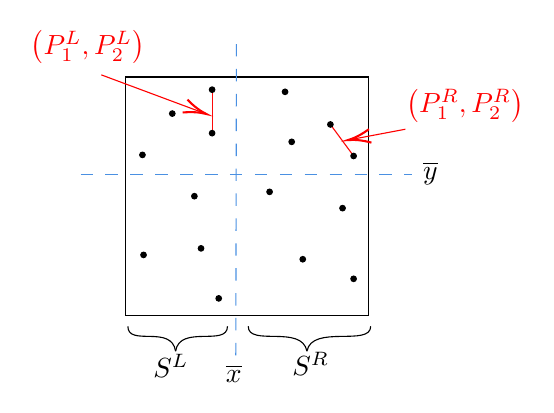
\begin{tikzpicture}[x=0.75pt,y=0.75pt,yscale=-1,xscale=1]
			%uncomment if require: \path (0,325); %set diagram left start at 0, and has height of 325

			%Shape: Rectangle [id:dp6499204868826074] 
			\draw   (80.93,157.92) -- (198.12,157.92) -- (198.12,272.62) -- (80.93,272.62) -- cycle ;
			%Straight Lines [id:da837478004805259] 
			\draw [color={rgb, 255:red, 74; green, 144; blue, 226 }  ,draw opacity=1 ] [dash pattern={on 4.5pt off 4.5pt}]  (59.2,204.85) -- (219,204.85) ;
			%Straight Lines [id:da7194776025159269] 
			\draw [color={rgb, 255:red, 74; green, 144; blue, 226 }  ,draw opacity=1 ] [dash pattern={on 4.5pt off 4.5pt}]  (134.31,142) -- (134,295) ;


			\draw [color={rgb, 255:red, 253; green, 10; blue, 10 }  ,draw opacity=1 ]   (122.59,164) -- (122.59,184.95) ;
			%Straight Lines [id:da715666979908854] 
			\draw [color={rgb, 255:red, 253; green, 10; blue, 10 }  ,draw opacity=1 ]   (179.58,180.76) -- (190.77,195.95) ;
			%Straight Lines [id:da6970165255401948] 
			\draw [color={rgb, 255:red, 255; green, 0; blue, 0 }  ,draw opacity=1 ]   (215.7,183.06) -- (189.96,187.93) ;
			\draw [shift={(188,188.3)}, rotate = 349.29] [color={rgb, 255:red, 255; green, 0; blue, 0 }  ,draw opacity=1 ][line width=0.75]    (10.93,-3.29) .. controls (6.95,-1.4) and (3.31,-0.3) .. (0,0) .. controls (3.31,0.3) and (6.95,1.4) .. (10.93,3.29)   ;
			%Straight Lines [id:da5840245566165858] 
			\draw [color={rgb, 255:red, 255; green, 0; blue, 0 }  ,draw opacity=1 ]   (69.21,156.87) -- (117.94,175.03) ;
			\draw [shift={(119.82,175.73)}, rotate = 200.44] [color={rgb, 255:red, 255; green, 0; blue, 0 }  ,draw opacity=1 ][line width=0.75]    (10.93,-3.29) .. controls (6.95,-1.4) and (3.31,-0.3) .. (0,0) .. controls (3.31,0.3) and (6.95,1.4) .. (10.93,3.29)   ;
			%Shape: Free Drawing [id:dp8916770831600931] 
			\filldraw (103.41,175.52) circle (1pt) ;
			%Shape: Free Drawing [id:dp7205705113694219] 
			\filldraw (179.58,180.76) circle (1pt);
			%Shape: Free Drawing [id:dp5723003936317532] 
			\filldraw (166.27,245.7) circle (1pt);
			%Shape: Free Drawing [id:dp19778776200558257] 
			\filldraw (89.56,243.61) circle (1pt);
			%Shape: Free Drawing [id:dp22218199289458562] 
			\filldraw (150.29,213.23) circle (1pt);
			%Shape: Free Drawing [id:dp9270216931653172] 
			\filldraw (157.74,165.04) circle (1pt);
			%Shape: Free Drawing [id:dp30577755696643694] 
			\filldraw (89.03,195.42) circle (1pt);
			%Shape: Free Drawing [id:dp8352617777328899] 
			\filldraw (125.78,264.56) circle (1pt);
			%Shape: Free Drawing [id:dp007121195742592068] 
			\filldraw (190.77,255.13) circle (1pt);
			%Shape: Free Drawing [id:dp9787419741468635] 
			\filldraw (160.94,189.14) circle (1pt);
			%Shape: Free Drawing [id:dp05782734388952204] 
			\filldraw (114.06,215.32) circle (1pt);
			%Shape: Free Drawing [id:dp020809307556031387] 
			\filldraw (122.59,184.95) circle (1pt);
			%Shape: Free Drawing [id:dp9236450749534464] 
			\filldraw (117.26,240.46) circle (1pt);
			%Shape: Free Drawing [id:dp9814876804759312] 
			\filldraw (185.44,221.08) circle (1pt);
			%Shape: Free Drawing [id:dp32677091280799897] 
			\filldraw (190.77,195.95) circle (1pt);
			%Shape: Free Drawing [id:dp7375869135394859] 
			\filldraw (122.59,164) circle (1pt) ;
			%Straight Lines [id:da2008032684012] 
			%Curve Lines [id:da7178341035011966] 
			\draw    (82,278) .. controls (82,288) and (103,277) .. (105,290) ;
			%Curve Lines [id:da31697667567298216] 
			\draw    (130,278) .. controls (130,288) and (107,277) .. (105,290) ;
			%Curve Lines [id:da6058144347191174] 
			\draw    (140,278) .. controls (140,288) and (165.81,277) .. (168.27,290) ;
			%Curve Lines [id:da842179996151678] 
			\draw    (199,278) .. controls (199,288) and (170.73,277) .. (168.27,290) ;

			% Text Node
			\draw (223,197.4) node [anchor=north west][inner sep=0.75pt]    {$\overline{y}$};
			% Text Node
			\draw (128,295.4) node [anchor=north west][inner sep=0.75pt]    {$\overline{x}$};
			% Text Node
			\draw (215,162.4) node [anchor=north west][inner sep=0.75pt]  [color={rgb, 255:red, 255; green, 0; blue, 0 }  ,opacity=1 ]  {$\left( P_{1}^{R} ,P_{2}^{R}\right)$};
			% Text Node
			\draw (34,134.4) node [anchor=north west][inner sep=0.75pt]  [color={rgb, 255:red, 255; green, 0; blue, 0 }  ,opacity=1 ]  {$\left( P_{1}^{L} ,P_{2}^{L}\right)$};
			% Text Node
			\draw (93,290.4) node [anchor=north west][inner sep=0.75pt]    {$S^{L}$};
			% Text Node
			\draw (160,289.4) node [anchor=north west][inner sep=0.75pt]    {$S^{R}$};


		\end{tikzpicture}


	\end{minipage}
\end{center}

\subsection{Conquer} Now we will recursively get the pair of closest points in $S_L$ and $S_R$. Suppose the $(P_1^L,P_2^L)$ are the closest pair of points in $S^L$ and $(P_1^R,P_2^R)$ are the closest pair of points in $S^R$.

\begin{algorithm}[H]
	\DontPrintSemicolon
	\SetKwProg{Fn}{Function}{:}{}
	\Fn{Conquer}{
		Solve for $S_L,S^R$.\;
		$(P_1^L,P_2^L)$ are the closest pair of points in $S_L$.\;
		$(P_1^R,P_2^R)$ are the closest pair of points in $S_R$.\;
		$\delta^L=d(P_1^L,P_2^L)$, $\delta^R=d(P_1^R,P_2^R)$\;
		$\delta_{min}\longleftarrow \min \{\delta^L,\delta^R\}$
	}
	\caption{Step 1 (Solve Subproblems)}
\end{algorithm}

\subsection{Combine}     Now we want to combine these two solutions.
\begin{question}{We are not done}{}
	Is there a pair of points $P_i,P_j\in S$ such that $d(P_i,P_j)<\delta_{min}$
\end{question}
If Yes: \begin{itemize}
	\item One of them must be in $S_L$ and the other is in $S_R$.
	\item $x-$coordinate $\in [\ovx-\delta_{min},\ovx+\delta_{min}]$.
	\item $|y_i-y_j|\leq \delta_{min}$
\end{itemize}
\parinf

So we take the strip of radius $\delta_{min}$ around $\ovx$. Define $T=\{P_i\in S\mid |x_i-\ovx|\leq \delta_{min}\}$

\begin{center}

	\tikzset{every picture/.style={line width=0.75pt}} %set default line width to 0.75pt        

	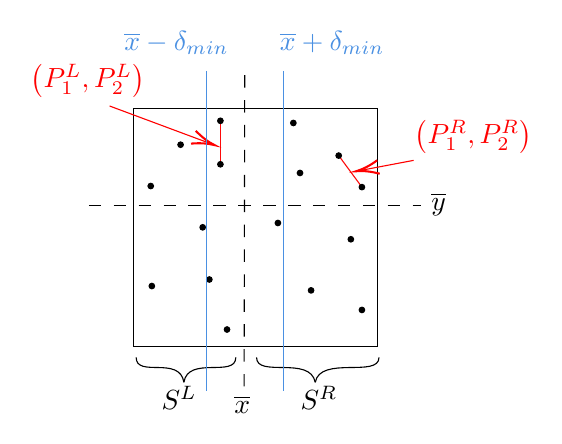
\begin{tikzpicture}[x=0.75pt,y=0.75pt,yscale=-1,xscale=1]
		%uncomment if require: \path (0,325); %set diagram left start at 0, and has height of 325

		%Shape: Rectangle [id:dp6499204868826074] 
		\draw   (80.93,157.92) -- (198.12,157.92) -- (198.12,272.62) -- (80.93,272.62) -- cycle ;
		%Straight Lines [id:da837478004805259] 
		\draw [color={rgb, 255:red, 0; green, 0; blue, 0 }  ,draw opacity=1 ] [dash pattern={on 4.5pt off 4.5pt}]  (59.2,204.85) -- (219,204.85) ;
		%Straight Lines [id:da7194776025159269] 
		\draw [color={rgb, 255:red, 0; green, 0; blue, 0 }  ,draw opacity=1 ] [dash pattern={on 4.5pt off 4.5pt}]  (134.31,142) -- (134,295) ;
		%Straight Lines [id:da2008032684012] 
		\draw [color={rgb, 255:red, 253; green, 10; blue, 10 }  ,draw opacity=1 ]   (122.59,164) -- (122.59,184.95) ;
		%Straight Lines [id:da715666979908854] 
		\draw [color={rgb, 255:red, 253; green, 10; blue, 10 }  ,draw opacity=1 ]   (179.58,180.76) -- (190.77,195.95) ;
		%Straight Lines [id:da6970165255401948] 
		\draw [color={rgb, 255:red, 255; green, 0; blue, 0 }  ,draw opacity=1 ]   (215.7,183.06) -- (189.96,187.93) ;
		\draw [shift={(188,188.3)}, rotate = 349.29] [color={rgb, 255:red, 255; green, 0; blue, 0 }  ,draw opacity=1 ][line width=0.75]    (10.93,-3.29) .. controls (6.95,-1.4) and (3.31,-0.3) .. (0,0) .. controls (3.31,0.3) and (6.95,1.4) .. (10.93,3.29)   ;
		%Straight Lines [id:da5840245566165858] 
		\draw [color={rgb, 255:red, 255; green, 0; blue, 0 }  ,draw opacity=1 ]   (69.21,156.87) -- (117.94,175.03) ;
		\draw [shift={(119.82,175.73)}, rotate = 200.44] [color={rgb, 255:red, 255; green, 0; blue, 0 }  ,draw opacity=1 ][line width=0.75]    (10.93,-3.29) .. controls (6.95,-1.4) and (3.31,-0.3) .. (0,0) .. controls (3.31,0.3) and (6.95,1.4) .. (10.93,3.29)   ;
		%Shape: Free Drawing [id:dp8916770831600931] 
		\filldraw (103.41,175.52) circle (1pt);
		%Shape: Free Drawing [id:dp7205705113694219] 
		\filldraw (179.58,180.76) circle (1pt);
		%Shape: Free Drawing [id:dp5723003936317532] 
		\filldraw (166.27,245.7) circle (1pt);
		%Shape: Free Drawing [id:dp19778776200558257] 
		\filldraw (89.56,243.61) circle (1pt);
		%Shape: Free Drawing [id:dp22218199289458562] 
		\filldraw (150.29,213.23) circle (1pt);
		%Shape: Free Drawing [id:dp9270216931653172] 
		\filldraw (157.74,165.04) circle (1pt);
		%Shape: Free Drawing [id:dp30577755696643694] 
		\filldraw (89.03,195.42) circle (1pt);
		%Shape: Free Drawing [id:dp8352617777328899] 
		\filldraw (125.78,264.56) circle (1pt);
		%Shape: Free Drawing [id:dp007121195742592068] 
		\filldraw (190.77,255.13) circle (1pt);
		%Shape: Free Drawing [id:dp9787419741468635] 
		\filldraw (160.94,189.14) circle (1pt);
		%Shape: Free Drawing [id:dp05782734388952204] 
		\filldraw (114.06,215.32) circle (1pt);
		%Shape: Free Drawing [id:dp020809307556031387] 
		\filldraw (122.59,184.95) circle (1pt);
		%Shape: Free Drawing [id:dp9236450749534464] 
		\filldraw (117.26,240.46) circle (1pt);
		%Shape: Free Drawing [id:dp9814876804759312] 
		\filldraw (185.44,221.08) circle (1pt);
		%Shape: Free Drawing [id:dp32677091280799897] 
		\filldraw (190.77,195.95) circle (1pt);
		%Shape: Free Drawing [id:dp7375869135394859] 
		\filldraw (122.59,164) circle (1pt);
		%Curve Lines [id:da7178341035011966] 
		\draw    (82,278) .. controls (82,288) and (103,277) .. (105,290) ;
		%Curve Lines [id:da31697667567298216] 
		\draw    (130,278) .. controls (130,288) and (107,277) .. (105,290) ;
		%Curve Lines [id:da6058144347191174] 
		\draw    (140,278) .. controls (140,288) and (165.81,277) .. (168.27,290) ;
		%Curve Lines [id:da842179996151678] 
		\draw    (199,278) .. controls (199,288) and (170.73,277) .. (168.27,290) ;
		%Straight Lines [id:da01763770038587964] 
		\draw [color={rgb, 255:red, 74; green, 144; blue, 226 }  ,draw opacity=1 ]   (153,140) -- (153,294) ;
		%Straight Lines [id:da6702110585391772] 
		\draw [color={rgb, 255:red, 74; green, 144; blue, 226 }  ,draw opacity=1 ]   (116,140) -- (116,294) ;

		% Text Node
		\draw (223,197.4) node [anchor=north west][inner sep=0.75pt]    {$\overline{y}$};
		% Text Node
		\draw (128,295.4) node [anchor=north west][inner sep=0.75pt]    {$\overline{x}$};
		% Text Node
		\draw (215,162.4) node [anchor=north west][inner sep=0.75pt]  [color={rgb, 255:red, 255; green, 0; blue, 0 }  ,opacity=1 ]  {$\left( P_{1}^{R} ,P_{2}^{R}\right)$};
		% Text Node
		\draw (30,135.4) node [anchor=north west][inner sep=0.75pt]  [color={rgb, 255:red, 255; green, 0; blue, 0 }  ,opacity=1 ]  {$\left( P_{1}^{L} ,P_{2}^{L}\right)$};
		% Text Node
		\draw (93,290.4) node [anchor=north west][inner sep=0.75pt]    {$S^{L}$};
		% Text Node
		\draw (160,290.4) node [anchor=north west][inner sep=0.75pt]    {$S^{R}$};
		% Text Node
		\draw (150,119.4) node [anchor=north west][inner sep=0.75pt]  [color={rgb, 255:red, 74; green, 144; blue, 226 }  ,opacity=1 ]  {$\overline{x} +\delta _{min}$};
		% Text Node
		\draw (75,119.4) node [anchor=north west][inner sep=0.75pt]  [color={rgb, 255:red, 74; green, 144; blue, 226 }  ,opacity=1 ]  {$\overline{x} -\delta _{min}$};


	\end{tikzpicture}
\end{center}
We now sort all the points in the $T$ by their decreasing $y-$coordinate. Let $T_y$ be the array of points. For each $P_i\in T_y$ define the region $$T_i=\{P_j\in T_y \mid 0\leq y_j-y_i\leq \delta_{min}, j>i\}$$

\pagebreak
\begin{center}
	\begin{minipage}{0.7\textwidth}

		\begin{lemma}{}{}
			Number of points (other than $P_i$) that lie inside the box is at most 8
		\end{lemma}
		\begin{proof}
			Suppose there are more than 8 points that lie inside the box apart from $P_i$. The box has a left square part and a right square part. So one of the squares contains at least 5 points. WLOG suppose the left square has at least 5 points. Divide each square into 4 parts by a middle vertical and a middle horizontal line. Now since there are 5 points there is one part which contains 2 points, but that is not possible as those two points are in $S_L$ and their distance will be less than $\delta_{min}$ which is not possible. Hence, contradiction. Therefore, there are at most 8 points inside the box.
		\end{proof}\parinn

		Hence by the above lemma for each $P_i\in T_y$ there are at most 8 points in $T_i$. So for each $P_j\in T_i$ we find the $d(P_i,P_j)$ and if it is less than $\delta_{min}$ we update the points and the distance
	\end{minipage}
	\hspace{1cm}
	\begin{minipage}{0.229\textwidth}



		\tikzset{every picture/.style={line width=0.75pt}} %set default line width to 0.75pt        

		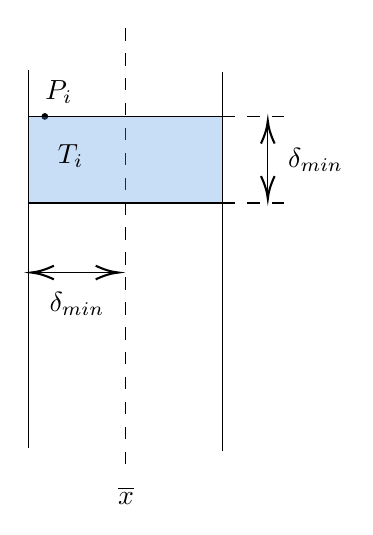
\begin{tikzpicture}[x=0.75pt,y=0.75pt,yscale=-1,xscale=1]
			%uncomment if require: \path (0,300); %set diagram left start at 0, and has height of 300

			%Straight Lines [id:da3975720681427135] 
			\draw    (200,50.92) -- (200,233.14) ;
			%Straight Lines [id:da42362227502058447] 
			\draw    (293.43,51.98) -- (293.43,234.2) ;
			%Straight Lines [id:da04130491026490812] 
			\draw  [dash pattern={on 4.5pt off 4.5pt}]  (246.71,30.67) -- (246.71,244.38) ;
			%Straight Lines [id:da4384742510539741] 
			\draw    (200,73.3) -- (293.43,73.3) ;
			%Straight Lines [id:da3745552754160917] 
			\draw    (200,114.85) -- (293.43,114.85) ;
			%Straight Lines [id:da9873374520652576] 
			\draw    (203.43,148.38) -- (241.43,148.38) ;
			\draw [shift={(243.43,148.38)}, rotate = 180] [color={rgb, 255:red, 0; green, 0; blue, 0 }  ][line width=0.75]    (10.93,-3.29) .. controls (6.95,-1.4) and (3.31,-0.3) .. (0,0) .. controls (3.31,0.3) and (6.95,1.4) .. (10.93,3.29)   ;
			\draw [shift={(201.43,148.38)}, rotate = 0] [color={rgb, 255:red, 0; green, 0; blue, 0 }  ][line width=0.75]    (10.93,-3.29) .. controls (6.95,-1.4) and (3.31,-0.3) .. (0,0) .. controls (3.31,0.3) and (6.95,1.4) .. (10.93,3.29)   ;
			%Straight Lines [id:da5826410245797784] 
			\draw    (315.43,77.3) -- (315.43,110.85) ;
			\draw [shift={(315.43,112.85)}, rotate = 270] [color={rgb, 255:red, 0; green, 0; blue, 0 }  ][line width=0.75]    (10.93,-3.29) .. controls (6.95,-1.4) and (3.31,-0.3) .. (0,0) .. controls (3.31,0.3) and (6.95,1.4) .. (10.93,3.29)   ;
			\draw [shift={(315.43,75.3)}, rotate = 90] [color={rgb, 255:red, 0; green, 0; blue, 0 }  ][line width=0.75]    (10.93,-3.29) .. controls (6.95,-1.4) and (3.31,-0.3) .. (0,0) .. controls (3.31,0.3) and (6.95,1.4) .. (10.93,3.29)   ;
			%Straight Lines [id:da8728720299963784] 
			\draw  [dash pattern={on 4.5pt off 4.5pt}]  (293.43,73.3) -- (329.43,73.3) ;
			%Straight Lines [id:da06933695064552192] 
			\draw  [dash pattern={on 4.5pt off 4.5pt}]  (293.43,114.85) -- (324.43,114.85) ;
			%Shape: Free Drawing [id:dp435305414025839] 
			\filldraw (208,73.17) circle (1pt) ;
			%Shape: Rectangle [id:dp914080675609527] 
			\draw  [fill={rgb, 255:red, 74; green, 144; blue, 226 }  ,fill opacity=0.3 ] (200,73.3) -- (293.43,73.3) -- (293.43,114.85) -- (200,114.85) -- cycle ;

			% Text Node
			\draw (209,156.4) node [anchor=north west][inner sep=0.75pt]    {$\delta _{min}$};
			% Text Node
			\draw (324,87.4) node [anchor=north west][inner sep=0.75pt]    {$\delta _{min}$};
			% Text Node
			\draw (207,54.4) node [anchor=north west][inner sep=0.75pt]    {$P_{i}$};
			% Text Node
			\draw (242,250.4) node [anchor=north west][inner sep=0.75pt]    {$\overline{x}$};
			% Text Node
			\draw (213,85.4) node [anchor=north west][inner sep=0.75pt]    {$T_{i}$};


		\end{tikzpicture}
	\end{minipage}
\end{center}
\subsection{Pseudocode and Time Complexity}
\begin{assumption*}
	We will assume for now that for all $P_i.P_j\in S$ we have $x_i\neq x_j$ and $y_i\neq y_j$. Later we will modify the pseudocode to remove this assumption
\end{assumption*}
\begin{algorithm}
	\DontPrintSemicolon
	\KwIn{Set of $n$ points, $S=\{(x_i,y_i)\mid x_i,y_i\in\bbR, \ \forall\ i\in[n]\}$. We denote $P_i=(x_i,y_i)$. }
	\KwOut{Closest pair of ponts, $(P_i,P_j,\delta)$ where $\delta=d(P_i,P_j)$}
	\Begin{
		\If{$|S|\leq 10$}{Solve by Brute Force (Consider every pair of points)}

		$S^x\longleftarrow S$ sorted by $x-$coordinate, \hspace{5mm} $S^y\longleftarrow S$ sorted by $y-$coordinate\;
		$\ovx\longleftarrow \lfloor \frac{n}{2}\rfloor $ highest $x-$coordinate, \hspace{5mm} $\ovy\longleftarrow \lfloor \frac{n}{2}\rfloor $ highest $y-$coordinate\;
		$S^L\longleftarrow \{P_i\mid x_i<\bar{x},\ \forall\ i\in[n]\}$, \hspace{5mm} $S^R\longleftarrow \{P_i\mid x_i\geq\bar{x},\ \forall\ i\in[n]\}$\;
		$(P_1^L,P_2^L,\delta^L)\longleftarrow$ \textsc{Find-Closest}($S^L$), \hspace{5mm} $(P_1^R,P_2^R,\delta^R)\longleftarrow$ \textsc{Find-Closest}($S^R$)\;
		$\delta_{min}\longleftarrow \min\{\delta^L,\delta^R\}$\;
		\If{$\delta_{min}<\delta^L$}{$P_1\longleftarrow P_1^R$, $P_2\longleftarrow P_2^R$}

		\Else{$P_1\longleftarrow P_1^L$, $P_2\longleftarrow P_2^L$}
		$T\longleftarrow \{P_i\mid |x_i-\ovx|\leq \delta_{min}\}$\;
		$T_y\longleftarrow T$ sorted by decreasing $y-$coordinate\;
		\For{$P\in T_y$}{
			$U\longleftarrow $ Next $8$ points\;
			\For{$\hat{P}\in U$}{
				\If{$d(P,\hat{P})<\delta_{min}$}{$\delta_{min}\longleftarrow d(P,\hat{P})$\;
					$(P_1,P_2)\longleftarrow (P,\hat{P})$}
			}
		}
		\Return{$(P_1,P_2,\delta_{min})$}
	}

	\caption{\textsc{Find-Closest}($S$)}
	\label{find-closest-nlog2n}
\end{algorithm}

Notice we used the assumption in the line $5$ for finding the medians. So the line 4 takes $O(n\log n)$ times. Lines 5,6 takes $O(n)$ time. Since $\ovx$ is the median, we have  $|S^L|=\lfloor \frac{n}2\rfloor$ and $|S^R|=\lceil \frac{n}{2}\rceil$. Hence $\textsc{Find-Closest}(S^L)$ and $\textsc{Find-Closest}(S^R)$ takes $T\lt(\frac{n}{2}\rt)$ time. Now lines $8-12$ takes constant time. Line 13 takes $O(n)$ time. And line 14 takes $O(n\log n)$ time. Since $U$ has 8 points i.e. constant number of points the lines $16-20$ takes constant time for each $P\in T_y$. Hence the for loop at line 15 takes $O(n)$ time. Hence total time taken $$T(n)=O(n)+O(n\log n)+2T\lt(\frac{n}2\rt)\implies T(n)=O(n\log^2n)$$
\section{Improved Algorithm for \texorpdfstring{$O(n\log n)$}{O(nlogn)} Runtime}
Notice once we sort the points by $x-$coordinate and $y-$coordinate we don't need to sort the points anymore. We can just pass the sorted array of points into the arguments for solving the smaller problems. Their is another time where we need to sort which is in line 14 of the above algorithm. This we can get actually from $S^y$ without sorting just checking one by one backwards direction if the $x-$coordinate of the points satisfy $|x_i-\ovx|\leq \delta_{min}$. So $$T_y=\textsc{Reverse}(\{P_i\in S^y\mid |x_i-\ovx|\leq \delta_{min}\})$$

So we form a new algorithm which takes the input $S^x$ and $S^y$ and then finds the closest pair of points. Then we will use that subroutine to find closest pair of points in any given set of points.

\begin{center}
	\begin{minipage}{0.55\textwidth}
		\begin{algorithm}[H]
			\DontPrintSemicolon
			\KwIn{Set of $n$ points, $S=\{(x_i,y_i)\mid x_i,y_i\in\bbR, \ \forall\ i\in[n]\}$.
				$S^x$ and $S^y$ are the sorted  array of points with respect to $x-$coordinate and $y-$coordinate respectively}
			\KwOut{Closest pair of ponts, $(P_i,P_j,\delta)$ where $\delta=d(P_i,P_j)$}
			\Begin{
				\If{$|S|\leq 10$}{Solve by Brute Force}

				$\ovx\longleftarrow \lfloor \frac{n}{2}\rfloor $ highest $x-$coordinate\;
				$\ovy\longleftarrow \lfloor \frac{n}{2}\rfloor $ highest $y-$coordinate\;
				$S^L\longleftarrow \{P_i\in S^x\mid x_i<\bar{x},\ \forall\ i\in[n]\}$\;
				$S^L_y\longleftarrow \{P_i\in S^y\mid x_i<\ovx\}$\;
				$S^R\longleftarrow \{P_i\in S^x\mid x_i\geq\bar{x},\ \forall\ i\in[n]\}$\;
				$S^R_y\longleftarrow \{P_i\in S^y\mid x_i\geq \ovx\}$\;
				$(P_1^L,P_2^L,\delta^L)\longleftarrow$ \textsc{Find-Closest-Sorted}($S^L,S^L_y$)\;
				$(P_1^R,P_2^R,\delta^R)\longleftarrow$ \textsc{Find-Closest-Sorted}($S^R,S^R_y$)\;
				$\delta_{min}\longleftarrow \min\{\delta^L,\delta^R\}$\;
				\If{$\delta_{min}<\delta^L$}{$P_1\longleftarrow P_1^R$, $P_2\longleftarrow P_2^R$}

				\Else{$P_1\longleftarrow P_1^L$, $P_2\longleftarrow P_2^L$}
				$T\longleftarrow \{P_i\mid |x_i-\ovx|\leq \delta_{min}\}$\;
				$T_y\longleftarrow \textsc{Reverse}(\{P_i\in S^y\mid |x_i-\ovx|\leq \delta_{min}\})$\;
				\For{$P\in T_y$}{
					$U\longleftarrow $ Next $8$ points\;
					\For{$\hat{P}\in U$}{
						\If{$d(P,\hat{P})<\delta_{min}$}{$\delta_{min}\longleftarrow d(P,\hat{P})$\;
							$(P_1,P_2)\longleftarrow (P,\hat{P})$}
					}
				}
				\Return{$(P_1,P_2,\delta_{min})$}
			}

			\caption{\textsc{Find-Closest-Sorted}($S^x,S^y$)}
			\label{find-closest-nlog2n-full}
		\end{algorithm}
	\end{minipage}
	\hspace{0.1mm}
	\begin{minipage}{0.43\textwidth}
		\begin{algorithm}[H]
			\DontPrintSemicolon
			\KwIn{Set of $n$ points, $S=\{(x_i,y_i)\mid x_i,y_i\in\bbR, \ \forall\ i\in[n]\}$. We denote $P_i=(x_i,y_i)$. }
			\KwOut{Closest pair of ponts, $(P_i,P_j,\delta)$ where $\delta=d(P_i,P_j)$}
			\Begin{
				\If{$|S|\leq 10$}{Solve by Brute Force}
				$S^x\longleftarrow S$ sorted by $x-$coordinate\;
				$S^y\longleftarrow S$ sorted by $y-$coordinate\;
				\Return{\textsc{Find-Closest-Sorted}$(S^x,S^y)$}
			}
			\caption{\textsc{Find-Closest}($S$)}
		\end{algorithm}
	\end{minipage}
\end{center}


This algorithm only sorts one time. So time complexity for $\textsc{Find-Closest-Sorted}(S^x,S^y)$ is $$T(n)=2T\lt(\frac{n}{2}\rt)+O(n)\implies T(n)=O(n\log n)$$and therefore times complexity for $\textsc{Find-Closest}(S)$ is $O(n\log n)$.

\section{Removing the Assumption}
For this there nothing much to do. For finding the median $\ovx$ if we have more than one points with same $x-$coordinate which appears as the $\lt\lfloor \frac{n}{2}\rt\rfloor$ highest $x-$coordinate we sort only those points with respect to their $y-$coordinate update the $S^x$ like that and then take $\lt\lfloor \frac{n}{2}\rt\rfloor$ highest point in $S^x$. We do the same for $S^y$ and update accordingly. All this we do so that $S^L$ and $S^R$ has the size $\frac{n}{2}$.

%\chapter{Median Finding in Linear Time}

\begin{algoprob}
	\problemtitle{\textsc{Median-Find}($S$)}
	\probleminput{Set $S$ of $n$ distinct integers}
	\problemquestion{Find the $\lt\lfloor\frac{n}{2}\rt\rfloor^{th}$ smallest integer in $S$}
\end{algoprob}

\section{Naive Algorithm}
The naive algorithm for this will be to sort the array in $O(n\log n)$ time then return the  $\lt\lfloor\frac{n}{2}\rt\rfloor^{th}$ element. This will take $O(n\log n)$ time. But in the next section we will show a linear time algorithm.

\section{Linear Time Algorithm}
In this section we will show an algorithm to find the median of a given set of distinct integers in $O(n)$ time complexity. We will follow \cite[Section 9.3]{CormenThomasLeisersonCharlesRivestRonaldSteinClifford_BOOK}. Consider the following two problems:

\begin{algoprob}
	\problemtitle{\textsc{Rank-Find} ($S,k$)}
	\probleminput{Set $S$ of $n$ distinct integers and an integer $k\leq n$}
	\problemquestion{Find the $k^{th}$ smallest integer in $S$}
\end{algoprob}
\begin{algoprob}
	\problemtitle{\textsc{Approximate-Split}($S$)}
	\probleminput{Set $S$ of $n$ distinct integers}
	\problemquestion{Given $S$, return an integer $z\in S$ such that $z$ where $rank(z)\in \lt[\frac{n}{4},\frac{3n}{4}\rt]$}
\end{algoprob}

%Certainly \prb{Rank-Find}$(S,k)$ is harder than $\prb{Approximate-Split}$. 
\subsection{Solve \prb{Rank-Find} using \prb{Approximate-Split}}
%Here suppose we can solve $\prb{Approximate-Split}$ easily. Now we want to solve $\prb{Rank-Find}$ using $\prb{Approximate-Split}$.
\begin{algorithm}
	\DontPrintSemicolon
	\KwIn{Set $S$ of $n$ distinct integer and $k\in[n]$}
	\KwOut{$k^{th}$ smallest integer in $S$}
	\Begin{
%$n\longleftarrow |S|$\;
\If{$|S|\leq 100$}{Sort $S$, \Return{$k^{th}$ smallest element in $S$}}	
$z\longleftarrow \prb{Approximate-Split}(S)$\hspace{1cm}
($z$ is the $r^{th}$ smallest element for some $r\in \lt[\frac{n}{4},\frac{3n}{4}\rt]$)\;
$S_L\longleftarrow \{x\in S\mid x\leq z\}$, $S_R\longleftarrow \{x\in S\mid x>z\}$\;
\If{$k\leq |S_L|$}{\Return{\prb{Rank-Find}$(S_L,k)$}}
\Return{\prb{Rank-Find}$(S_R,k-|S_L|)$}
}
\caption{\prb{Rank-Find}(S,k)}
\end{algorithm}
\parinn

Certainly if we can solve $\prb{Rank-Find}(S,k)$ for all $k\in[n]$ we can also solve $\prb{Median-Find}$. We will try to use both the problems and recurse to solve \prb{Rank-Find} in linear time. 

In the above algorithm $rank(z)\in \lt[\frac{n}{4},\frac{3n}{4}\rt]$. So $\frac{n}4\leq |S_L|,|S_R|\leq \frac{3n}4$. For now suppose $\prb{Rank-Find}(S,k)$ takes $T_{RF}(n)$ time and $\prb{Approximate-Split}(S)$ takes $T_{AS}(n)$ time. Then the time taken by the algorithm is  $$T_{RF}(n)\leq O(n)+T_{AS}(n)+T_{RF}\lt(\frac{3n}4\rt)$$
\subsection{Solve \prb{Approximate-Split} using \prb{Rank-FInd}}
We first divide $S$ into groups of $5$ elements. So take $t=\lt\lceil\frac{n}5\rt\rceil$. Now we sort each group. Since each group have constant size this can be done in $O(n)$ time. So now consider the scenario:
\begin{figure}[h]
	\centering
	\includegraphics{images/approx-split-using-rankfind}
\end{figure}
%\chapter{Polynomial Multiplication}
\begin{algoprob}
	\problemtitle{{Polynomial Multiplication}}
	\probleminput{Given 2 polynomials of degree $n-1$ by 2 arrays of their coefficients $(a_0,\dots, a_{n-1})$ and $(b_0,\dots, b_{n-1})$ such that $A(x)=a_0+a_1x+\cdots+ a_{n-1}x^{n-1}$ and $B(x)=b_0+b_1x+\cdots+b_{n-1}x^{n-1}$ respectively}
	\problemquestion{Given 2 polynomials of degree $n-1$ find their product polynomial of degree $2n-2$ by returning the array of their coefficients.}
\end{algoprob}
%\chapter{Dynamic Programming}
\section{Longest Increasing Subsequence}
\begin{algoprob}
	\problemtitle{\prb{Longest Increasing Subsequence}}
	\probleminput{Sequence of distinct integers $A=(a_1,\dots, a_n)$}
	\problemquestion{Given an array of distinct integers find the longest increasing subsequence i.e. return maximum size set $S\subseteq[n]$ such that $\forall\ i,j\in S$, $i<j\implies a_i<a_j$}
\end{algoprob}
\dfnc[dynamic-prog]{Dynamic Programming}{Dynamic Programming has 3 components:\begin{enumerate}
		\item {Optimal Substructure}: Reduce problem to smaller independent problems
		\item {Recursion}: Use recursion to solve the problems by solving smaller independent problems
		\item {Table Filling}: Use a table to store the result to solved smaller independent problems.
\end{enumerate}}
\subsection{$O(n^2)$ Time Algorithm}
Given $A=(a_1,\dots, a_n)$ first we will create a $n$-length array where $i^{th}$ entry stores the length and longest increasing subsequence ending at $a_i$. Certainly we have the following recursion relation$$\prb{LIS}(k)=1+\max\limits_{\substack{j<k,\  a_j<a_k}}\{\prb{LIS}(j)\}$$since if a subsequence $S\subseteq [n]$ is the longest increasing subsequence ending at $a_k$ then certainly $S-\{k\}$ is the longest increasing subsequence which ends at $a_j<a_k$ for some $j<k$. 

Hence in the table we start with 1st position and using the recursion relation we fill the table from left. And after the table is filled we look for which entry of the table has maximum length. So the algorithm will be following:

\begin{algorithm}\SetKwComment{Comment}{// }{}
	\DontPrintSemicolon
	\KwIn{Sequence of distinct integers $A=(a_1,\dots, a_n)$}
	\KwOut{Maximum size set $S\subseteq [n]$ such that $\forall\ i,j\in S$, $i<j\implies a_i<a_j$.}
	\Begin{
	Create an array $T$ of length $n$\;
	\For{$i\in[n]$}{
	$T[i][1]\longleftarrow 1+\max\{T[j][1]\colon j<k,\ a_j<a_k\}$\Comment*{Finds $\prb{LIS}[i]$}
$T[i][2]\longleftarrow T\big[T[i][1]-1\big][2]$
}	
$Index\longleftarrow \max \{T[j][1]\colon j\in[n]\}$\;
\Return{$T[Index]$}
}
\caption{\prb{LIS}$(A)$}
\end{algorithm}
\pagebreak 

For each iteration of the loop it takes $O(n)$ time to find $\prb{LIS}[i]$. Hence the time complexity of this algorithm is $O(n^2)$. 
\subsection{\texorpdfstring{$O(n\log n)$}{O(logn)} Time Algorithm}
In the following algorithm we update the longest increasing sequence every time we see a new element of the given sequence. At any time we keep the best available sequence.
\begin{algorithm}\SetKwComment{Comment}{// }{}
	\DontPrintSemicolon
	\KwIn{Sequence of distinct integers $A=(a_1,\dots, a_n)$}	
	\KwOut{Maximum size set $S\subseteq [n]$ such that $\forall\ i,j\in S$, $i<j\implies a_i<a_j$.}
\Begin{
	Create an array $T$ of length $n$ with all entries $0$\;
	Create an array $M$ of length $n$\;
	\For{$i=1,\dots, n$}{$M[i]\longleftarrow \infty$}	
	\For{$i=1,\dots,n$}{
		$k\longleftarrow $Find smallest index $i$ such that $M[k]>a_i$ using \prb{Binary-Search}\;
		$M[k]\longleftarrow i$\;
		$T[i]\longleftarrow M[k-1]$\Comment*{Pointer to the previous element of the sequence}
}
$l\longleftarrow $ Largest $l$ such that $M[l]$ is finite\;
Create an array $S$ of length $l$\;
\For{$i=l,\dots, 1$}{
	\If{$i=l$}{$S[l]\longleftarrow M[l]$\;
	Continue}
$S[i]\longleftarrow T\big[S[i+1]\big]$\Comment*{$T[S[i+1]]$ is pointer to previous value of sequence}
}
\Return{$(l,S)$}
}
\caption{\prb{QuickLIS}$(A)$}
\end{algorithm}\parinf

\textbf{Time Complexity:} To create the arrays and the first for loop takes $O(n)$ time. In each iteration of the for loop at line 6 it takes $O(\log n)$ time to find $k$ and rest of the operations in the loop takes constant time. So the for loop takes $O(n\log n)$ time.  Then To find $l$ and creating $S$ it takes $O(n)$ time. Then in the for loop at line 12 in each iteration it takes constant time. So the for loop at line 12 takes in total $O(n)$ time. Therefore the algorithm takes $O(n\log n)$ time. \parinn

We will do the proof of correctness of the algorithm now.
%\begin{example}{Working of algorithm}{}
%	\begin{align*}
%		&6,12,4,3,7,10,8,18,11,16,9\\
%		&\cancel{\infty}, \cancel{\infty}, \cancel{\infty}, \cancel{\infty}, \cancel{\infty}, \cancel{\infty}, \cancel{\infty},\dots \\
%		&\cancel{6},\cancel{12},\cancel{10},\cancel{18},\cancel{16}\\
%		& \cancel{4}, 7,8,\cancel{11}\\
%		& 3, \ \ \ 9
%	\end{align*}
%\end{example}


\begin{lemma}{}{mdecreasing}
	For any index $M[k]$ is non increasing
\end{lemma}
\begin{proof}
	Every time we change a value of $M[k]$ we replace by something smaller. So $M[k]$ is non increasing.
\end{proof}
We denote the state of array $M$ at $i^{th}$ iteration by $M^i$. Then we have the following lemma:

\begin{lemma}{}{}
At any time $i$, $M^i[1]\leq M^i[2]\leq \cdots\leq M^i[n]$
\end{lemma}
\begin{proof}
We will prove this by induction on $i$. The base case follows naturally. Now for $i^{th}$ iteration suppose $M^i[k]$ is replaced by $x_i$. Then we know $\forall \ j<k$ we have $M^i[j]\leq x_i$. By inductive hypothesis at time $t-1$ we have $M$ as an increasing sequence. Now before replacing $M^i[k]\leq M^i[k+1]\leq \cdots M^i[n]$. Now by \lmref{th:mdecreasing} $M^i[k]$ is nonincreasing. So  So we still have $M^i[1]\leq \cdots M^i[k-1]\leq x_i\leq M^i[k+1]\leq \cdots \leq M^i[n]$. Hence bt mathematical induction it holds.
\end{proof}

Now suppose at $i^{th}$ iteration $k_i$ is largest such that $M^i[k_i]<\infty$. Then $S^i$ denote the set constructed like the way we constructed at line 12--16 in the algorithm i.e. $$S^i[k_i]=M^i[k_i]\qquad \text{and}\qquad S^i[j]=T[S^i[j+1]]\quad \forall\ j\in[k_i-1]$$
\begin{lemma}{}{si-isgoodatalliterations}
	After any $i^{th}$ iteration, for $k\in[n]$ if $M^i[k]<\infty$ then $S^i[k]$ stores the smallest value in $x_1,\dots, x_i$ such that there is an increasing subsequence of size $k$ that ends in $S^i[k]$.
\end{lemma}
\begin{proof}
We will induction on $i$. Base case: This is true after first iteration since only $M^1[1]<\infty$. So this naturally follows. 

Suppose this is true after $i$ iterations.  Now at $(i+1)^{th}$ iteration suppose $t$ be the smallest index such that $M^i[t]>x_{i+1}$. Then we have $$M^i[1],\dots, M^i[t-1]<x_{i+1}<M^i[k],\dots, M^i[n]\implies S^i[1],\dots, S^i[t-1]<x_{i+1}<S^i[k],\dots, S^i[k_i]$$ Now for $k\leq t-1$ it is true by the inductive hypothesis. For $k>t$ and if $M^{i+1}[k]<\infty$ then $S^{i+1}[k]$ is the smallest value in $x_1,\dots, x_{i+1}$ such that there is an increasing subsequence of size $k$ that ends in $S^{i+1}[k]$ since this was true for $i^{th}$ iteration. 

Now only the case when $k=t$ is remaining. If $S^{i+1}[k]$ is not the smallest value in $x_1,\dots ,x_{i+1}$ to have an increasing subsequence of size $k$ ending at $S^{i+1}[k]$ then let $x_j$ was the smallest value to satisfy this condition where $j<i+1$. Then naturally $x_j<x_{i+1}$. Then $M^{i}[t]\leq x_j<x_{i+1}$. But we $t$ was the smallest number such that $M^{i}[t]>x_{i+1}$. Hence contradiction. Therefore $S^i[k]$ is the smallest value in $x_1,\dots, x_{i+1}$ to have an increasing subsequence of size $k$ ending at $S^{i+1}[k]$. 

Therefore by mathematical induction this is true for all iterations. 
\end{proof}

Now we will show that $S$ is indeed the longest increasing subsequence.


\begin{lemma}{}{}
	$S$ is the longest increasing subsequence of $A$.
\end{lemma}
\begin{proof}
	After the $n^{th}$ iteration $S^n=S$ and $k_n=l$. Hence by \lemref{th:si-isgoodatalliterations} we can say for all $k\in[l]$, $S[k]$ is the smallest number such that there is an increasing sequence of length $k$ ending at $S[k]$. Now we want to show that this increasing sequence is the longest increasing subsequence of $A$. Suppose $S$ is not the longest increasing subsequence. Let $T$ be the longest increasing subsequence of length $t$. Then suppose $j\leq l$ be the smallest index such that $S[j]\neq T[j]$. Now $S[j]$ is the smallest number in $x_1,\dots, x_n$ such that there is an increasing subsequence of length $j$ ending at $S[j]$. Hence we have $S[j]<T[j]$. Now for all $i<j$ we have $S[i]=T[i]$.   Then we form this new subsequence $$\hat{T}=\{T[1],T[2],\dots, T[j-1], S[j],T[j],\dots, T[t]\}$$Certainly $\hat{T}$ has length $t+1$ and it is also an increasing subsequence. But this contradicts the maximality condition of $T$. Hence $S$ is indeed the longest increasing subsequence.
\end{proof}

\section{Opimal Binary Search Tree}
%\chapter{Greedy Algorithm}

\section{Maximal Matching}

\begin{algoprob}
	\problemtitle{Maximal-Matching}
	\probleminput{Graph $G=(V,E)$}
	\problemquestion{Find a maximal matching $M\subseteq E$ of $G$}
\end{algoprob}
Before diving into the algorithm to find a matching or maximal matching we first define what is a matching.
\begin{Definition}{Matching}{}
	For a graph $G=(V,E)$ a matching $M\subseteq E$ is a set of edges such that no two edges in $M$ are incident on same vertex.
\end{Definition}
\begin{Definition}{Maximal Matching}{}
	For a graph $G=(V,E)$ a matching $M\subseteq E$ is maximal if it cannot be extended and still by adding an edge.
\end{Definition}
There is also a maximum matching which can be easily understood from the name:
\begin{Definition}{Maximum Matching}{}
	For a graph $G=(V,E)$ a matching $M\subseteq E$ is maximum if it is maximal and has the maximum size among all the maximal matchings.
\end{Definition}

\begin{idea*}
	The idea is to create a maximal matching we will just go over each edge one by one and check if after adding them to the set $M$  the matching property still holds. 
\end{idea*}
\begin{algorithm}
	\SetKwComment{Comment}{// }{}
	\DontPrintSemicolon
	\KwIn{Graph $G=(V,E)$}
	\KwOut{Maximal Matching $M\subseteq E$ of $G$}
	\Begin{
	$M\longleftarrow \emptyset$\;
	Order the edges $E=\{e_1,\dots, e_k\}$ arbitrarily\;
	\For{$e\in E$}{\If{$M\cup \{u\}$ is matching}{$M\longleftarrow M\cup \{e\}$}}
	\Return{$M$}	
}
\caption{\prb{Maximal-Matching}}
\end{algorithm}

\begin{question}{}{}
		Do we always get the largest possible matching?
\end{question}
\solve{ Clearly algorithm output is not optimal always. We get a maximal matching sure. But we don't get a maximum matching always. For example the following graph
	\begin{center}
		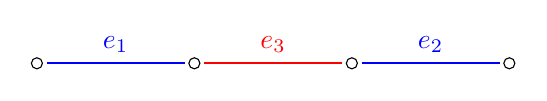
\begin{tikzpicture}
			\draw (-2,0) circle (2pt) node (A){};
			\draw (0,0) circle (2pt) node (B){};
			\draw (2,0) circle (2pt) node (C){};
			\draw (4,0) circle (2pt) node (D){};
			\draw[blue, thick] (A) -- node[midway, above]{$e_1$} (B);
			\draw[red, thick] (B) -- node[midway, above]{$e_3$}(C);
			\draw[blue, thick] (C) -- node[midway, above]{$e_2$} (D);
		\end{tikzpicture}
	\end{center}
	If we start from $e_1$ we get the matching $\{e_1.e_2\}$ which is maximum matching but if we start from $e_3$ then we get only the maximal matching $\{e_3\}$ which is not maximum.}

 Since the algorithm output may not be optimal always we can ask the following question
 \begin{question}{}{}
 	How large is the matching obtained compared to the maximum matching?
 \end{question}
This brings us to the following result:

\begin{Theorem}{}{}
	For any graph $G$ let the greedy algorithm obtains the matching $M$ and the maximum matching is $M^{\star}$. Then $$|M|\geq \frac12|M^\star|$$
\end{Theorem}
\begin{proof}
	Consider an edge $e\in M^{\star}$ but $e\notin M$. Since $e$ wasn't  picked in $M$, $\exs\ e'\in M\setminus M^{\star}$ such that $e$ and $e'$ are incident on same vertex. Thus define the function $f:M^{\star}\to M$ where $$f(e)=\begin{cases}
		e&\text{when $e\in M$}\\
		e' & \text{when $e\in M^{\star}\setminus M$ where $e'\in M\setminus M^{\star}$ such that $e'\cap e\neq \emptyset$}
	\end{cases}$$

Now note that there are at most  two edges in $M^{\star}$ that are adjacent to an edge $e'\in M$ which will be mapped to $e'$. Hence $$|M\setminus M^{\star}|\geq \frac12 |M^{\star}\setminus M|$$Therefore $|f^{-1}(e')|\leq 2$ $\forall\ e'\in M$. Hence $$|M^\star|=|M\cap M^{\star}|+|M^{\star}\setminus M|\leq |M\cap M^{\star}||+2|M\setminus M^{\star}|\leq 2|M|$$Therefore we have the result $|M|\geq \frac12|M^{\star}|$. 
\end{proof}
\begin{alternate-proof} 
	Let $M_1$ and $M_2$ are two matchings. Consider the symmetric difference $M_1\triangle M_2$.  This consists of edges that are in exactly one of $M_1$ and $M_2$. Now in $M\triangle M^{\star}$ we have the following properties:
	\begin{enumerate}[label=(\alph*)]
		\item Every vertex in $M\triangle M^{\star}$ has degree $\leq 2\implies $ Each component is a path or an even cycle. 
		\item The edges of $M$ and $M^{\star}$ alternate. 
			\end{enumerate}
		Now we will prove the following property about the connected components of $M\triangle M^{\star}$.
		
\begin{center}
					
	\begin{minipage}{0.9\textwidth}
			\textit{\textbf{Claim:}}\hspace{1em} No connected component is a single edge. 
		
		\begin{proof}
			This is because let $e$ be a connected component. So the two edges $e_1,e_2$ which are adjacent to $e$,  they are either in both $M$ and $M^{\star}$ or not in $M$ and $M^{\star}$. The former case is not possible because then $e_1,e_2,e$ are all in either $M$ or $M^{\star}$ which is not possible as they do not satisfy the condition of matching. For the later case since $M^{\star}$ is maximal matching, $e\in M^{\star}$. Then $e\notin M$. That means $e,e_1,e_2\notin M$ which is not possible since $M$ is also a maximal matching. Therefore no connected component is a single edge.
		\end{proof}
	\end{minipage}
\end{center}

	
		Therefore every path has length $\geq 2$. Therefore ratio of $\#$ edges of $M$ to $\#$ edges of $M^{\star}$ in a path is $\leq 2$. And for cycles we have $\#$ edges of $M=\#$ edges of $M^{\star}$. So in every connected component $C$ of $M\triangle M^{\star}$ the ratio $\frac{|M^{\star}\cap C|}{|M\cap C|}\leq 2$. Therefore we have $$\frac{|M^{\star}|}{|M|}=\frac{|M\cap M^{\star}|+\sum\limits_{C}|M^{\star}\cap C|}{|M\cap M^{\star}|+\sum\limits_{C}|M\cap C|}\leq 2$$Hence we have $|M|\geq \frac12|M^\star|$.
		

\end{alternate-proof}
\section{Huffman Encoding}
\begin{algoprob}
	\problemtitle{Huffman-Coding}
	\probleminput{$n$ symbols $A=(a-1,\dots, a_n)$ and their frequencies $P=(f_1,\dots, f_n)$ of using symbols}
	\problemquestion{Create a binary encoding such that: \begin{itemize}[itemsep=-0.2cm]
			\item Prefix Free: The code for one word can not be prefix for another code
			\item Minimality: Minimize $\prb{Cost}(b)=\sum\limits_{i=1}^n f_i\cdot \prb{Len}(b(a_i))$ where $b:A\to \{0,1\}^*$ is the binary encoding
	\end{itemize}}
\end{algoprob}

Assignment of binary strings can also be scene as placing the symbols in a binary tree where at any node $0$ means left child and $1$ means right child. Then the first condition implies that there can not be two codes which lies in the same path from the root to a leaf. I.e. it means that all the codes have to be in the leaves. Then the length of the binary coding for a symbol  is the height of the symbol in the binary tree. 

We can think the frequencies as the probability of appearing for a letter. We denote the probability of appearing of the letter $a_i$ by $p(a_i)\coloneqq \frac{f_i}{\sum\limits_{i=1}^nf_i}$. So the we can see the updated cost function $$\prb{Cost}(b)=\sum\limits_{i=1}^n p(a_i)\cdot\prb{Len}(b(a_i))$$And from now on we will see the frequencies as probabilities and cost function like this

\subsection{Optimal Binary Encoding Tree Properties}
Then our goal is to finding a binary tree with minimum cost where all the symbols are at the leaves. We have the following which establish the optimality of Huffman encoding over all prefix encodings where each symbol is assigned a unique string of bits.
\begin{lemma}{}{least-frequent-max-height}
	In the optimal encoding tree  least frequent element has maximum height.
\end{lemma}
\begin{proof}
	Suppose that is not the case. Let $T$ be the optimal encoding tree and let the least frequent element $x$ is at height $h_1$ and the element with the maximum height is $y$ with height $h_2$ and we have $h_1<h_2$.  Then we construct a new encoding tree $T'$ where we swap the positions of $x$ and $y$. So in $T'$ height of $y$ is $h_1$ and height of $x$ is $h_2$. Then $$\prb{Cost}(T)-\prb{Cost}(T')=(p(x)h_1+p(y)h_2)-(p(x)h_2+p(y)h_1)=(p(x)-p(y))(h_1-h_2)$$Since $p(x)<p(y)$ and $h_1<h_2$ we have $\prb{Cost}(T)-\prb{Cost}(T')>0$. But that is not possible since $T$ is the optimal encoding tree. So $T$ should have the minimum cost. Hence contradiction. $x$ has the maximum height.
\end{proof}

\begin{lemma}{}{complete-tree}
	The optimal encoding binary tree must be complete binary tree. (i.e. every non-leaf node has exactly $2$ children)
\end{lemma}
\begin{proof}
	Suppose $T$ be the optimal binary tree and there is a non-leaf node $r$ which has only one child at height $h$. 
	By \lmref{least-frequent-max-height} the least frequent element $x$ has the maximum height, $h_m$. 
	
	 Then consider the new tree $\hat{T}$ where we place the least frequent element at height $h$ and make it the second child of the node $r$. Then $$\prb{Cost}(T)-\prb{Cost}(\hat{T})=p(x)h_m-p(x)h=p(x)(h_m-h)>0$$But this is not possible as $T$ is the optimal binary tree and it has the minimal cost. Hence contradiction. Therefore the optimal encoding binary tree must be a complete binary tree. 
\end{proof}
\begin{lemma}{}{least-frequents-siblings}
There is an optimal binary encoding tree such that the least frequent element and the second least frequent element are siblings at the maximum height.
\end{lemma}
\begin{proof}
Let $T$ be optimal binary encoding tree. Suppose $x$, $y$ are the least frequent element and the second least frequent element. And suppose $b$, $c$  be two siblings at the maximum height of the tree (There may be many such siblings, and if so pick any such pair.). If $\{x,y\}=\{b,c\}$ we are done. So suppose not. Let the frequencies of $x,y,b,c$ are respectively $p(x),p(y),p(b),p(c)$ and heights of $x,y,b$ are $h_x,h_y$ and $h$ respectively.  WLOG assume $p(x)\leq p(y)$ and $p(b)\leq p(c)$. 

Now since we know $x,y$ have the smallest frequencies we have $p(x)\leq p(b)$ and $p(y)\leq p(c)$. And since $b,c$ have the maximum height we have $h_x,hy\geq h$. So we switch the position of $x$ with $b$ to form the new tree $T'$. And from $T'$ we swap the positions fo $y$ and $c$ to form a new tree $T''$.

\begin{center}
	\begin{tikzpicture}[
		every node/.style={font=\sffamily, align=center, line width=0.15mm},
		level 1/.style={level distance=1cm, sibling distance=2cm},  % Adjusted distance for level 1
		level 2/.style={sibling distance=2cm},   % Adjusted distance for level 2
		square/.style={draw, shape=rectangle, minimum width=0.5cm, minimum height=0.5cm, inner sep=0pt, text width=0.5cm, text centered},
		circle/.style={draw, shape=circle, minimum width=0.5cm, minimum height=0.5cm, inner sep=0pt, text width=0.5cm, text centered},
		filled/.style={fill=blue!20, , draw, line width=0.12mm},  % Style for filled nodes
		every edge/.style = {draw, latex'-latex' , line width=0.3mm, dotted,},
		parentarrow/.style={line width=0.12mm, -{latex[length=1mm, width=0.2mm, open, round]}},  % Style for arrows from nodes to children
		]
		
		% Leftmost tree
		\node[circle] (A1) {}
		child {node[circle] (B1) {}
			child {node[square] (D1) {$y$} edge from parent[parentarrow]}
			child {node[circle] (E1) {}
				child {node[square] (F1) {$c$} edge from parent[parentarrow]}
				child {node[square, filled] (G1) {$b$} edge from parent[parentarrow]}
				edge from parent[parentarrow]
			}
		edge from parent[parentarrow]
		}
		child {node[square,filled] (C1) {$x$} edge from parent[parentarrow]};
		\node[above left=0cm and 0cm of A1] (T1) {$T$};  % Label T1
		% Middle tree
		\node[circle, right=4cm of A1] (A2) {}
		child {node[circle] (B2) {}
			child {node[square, filled] (D2) {$y$} edge from parent[parentarrow]}
			child {node[circle] (E2) {}
				child {node[square, filled] (F2) {$c$} edge from parent[parentarrow]}
				child {node[square] (G2) {$x$} edge from parent[parentarrow]}
				edge from parent[parentarrow]
			}
			edge from parent[parentarrow]
		}
		child {node[square] (C2) {$b$} edge from parent[parentarrow]};
		\node[above left=0cm and 0cm of A2] (T1) {$T'$};  % Label T2
		
		% Rightmost tree
		\node[circle, right=4cm of A2] (A3) {}
		child {node[circle] (B3) {}
			child {node[square] (D3) {$c$}edge from parent[parentarrow]}
			child {node[circle] (E3) {}
				child {node[square] (F3) {$y$} edge from parent[parentarrow]}
				child {node[square] (G3) {$x$} edge from parent[parentarrow]}
				edge from parent[parentarrow]
			}
		edge from parent[parentarrow]
		}
		child {node[square] (C3) {$b$} edge from parent[parentarrow]};
		\node[above left=0cm and 0cm of A3] (T1) {$T''$};  % Label T3
		
		
		% Dotted bidirectional bent arrows between leaf nodes D and E in each tree
		\draw (C1) edge[bend left=45] (G1);
		\draw (F2) edge[bend left=45] (D2);
		
		% Arrows from leftmost tree to middle tree and from middle tree to rightmost tree
		\draw[-Latex, thick, shorten <= 1mm, shorten >= 1mm] (A1) -- (A2);
		\draw[-Latex, thick, shorten <= 1mm, shorten >= 1mm] (A2) -- (A3);
		
	\end{tikzpicture}
\captionof{figure}{Showing that the lowest probability nodes are siblings at the tree’s lowest level.} 
\label{fig:least-frequent-elm-siblings}
\end{center}

Now we will calculate how the cost changes as we go from $T$ to $T'$ and $T'$ to $T''$. First check for $T\to T'$. Almost all the nodes contribute the same except $x,b$. So we have $$\prb{Cost}(T)-\prb{Cost}(T')=(h_x\cdot p(x)+h\cdot p(b))-(h_x\cdot p(b)+h\cdot p(x))=(p(b)-p(x))(h-h_x)\geq 0$$Therefore swapping $x$ and $b$ does not increase the cost and since $T$ is the optimal binary encoding tree the cost doesn't decrease either. Therefore the costs are equal. Hence $T'$ is also an optimal tree. 

Similarly we calculate cost for going from $T'$ to $T''$ we have $$\prb{Cost}(T')-\prb{Cost}(T'')=(h_y\cdot p(y)+h\cdot p(c))-(h_y\cdot p(c)+h\cdot p(y))=(p(c)-p(y))(h-h_y)\geq 0$$Therefore swapping $y$ and $c$ also does not increase the cost and since $T'$ is the optimal binary encoding tree the cost doesn't decrease either. Therefore the costs are equal. Hence $T''$ is also an optimal tree. Hence $T''$ is the optimal tree where the least frequent element and second last frequent element are siblings.
\end{proof}




By the \lmref{complete-tree} and \lmref{least-frequents-siblings} we have that the least frequent element and the second least frequent element are siblings and they have the maximum height.

%\begin{Theorem}{}{replace-less-variable-case}
%Let $T_n$ be any optimal binary encoding tree following \lmref{least-frequents-siblings} (i.e. lowest probability symbols $x$ and $y$ are siblings at the deepest level). Let $T_{n-1}$ be the tree that results by replacing these two leaf nodes for $x,y$  and their parent with a single leaf node $z$ of probability $p(z)=p(x)+p(y)$. Then $$\prb{{Cost}}(T_n)=\prb{Cost}(T_{n-1})+p(z)$$
%\end{Theorem}
%\begin{proof}
%	Let $h$ be the heights of $x$ and $y$ in $T_n$. Clearly $z$ is in height $h-1$ in $T_{n-1}$. Since $z$ replaces $x$ and $y$ the costs of the two trees satisfies \begin{align*}
%		\prb{Cost}(T_n)&=\prb{Cost}(T_{n-1})-(\text{\prb{Cost} due to $z$ in \prb{Cost}$(T_{n-1})$} + (\text{\prb{Cost} due to $x$ and $y$ in \prb{Cost}$(T_{n})$})\\
%		& =\prb{Cost}(T_{n-1})-p(z)\cdot (d-1)+(p(x)+p(y))\cdot d\\
%		& = \prb{Cost}(T_{n-1})-p(z)\cdot (d-1)+p(z)\cdot d\\
%		& = \prb{Cost}(T_{n-1})+p(z)
%	\end{align*}
%\end{proof}

\begin{observation*}
	The cost of the trees $T_n$ and $T_{n-1}$ differ only by the fixed term $p(z)=p(x)+p(y)$ which does not depend on the tree's structure. Therefore minimizing the cost for $T_n$ is equivalent to minimizing the cost of $T_{n-1}$.
\end{observation*}
\begin{Theorem}{}{replace-less-variable-case}
	Given an instance with symbols $\mcI$: \begin{center}
		\begin{tabular}{ccccccccc}
			$a_1$, & $a_2$, & $\cdots$, & $a_i$, & $\cdots$, & $a_j$, & $\cdots$, & $a_n$ & with probabilities\\
			$p(a_1)$, & $p(a_2)$, & $\cdots$, & $p(a_i)$, & $\cdots$, & $p(a_j)$, & $\cdots$, & $p(a_n)$ &
		\end{tabular} 
	\end{center}
	such that $a_i$, $a_j$ are the least frequent and second least frequent elements respectively. Consider the instance with $n-1$ symbols $\mcI'$:
	\begin{center}
		\begin{tabular}{ccccccccccc}
			$a_1$, & $a_2$, & $\cdots$, & $a_{i-1}$, & $a_{i+1}$,& $\cdots$, & $a_{j-1}$,& $a_{j+1}$, & $\cdots$, & $a_n$, & $z$ \\
			$p(a_1)$, & $p(a_2)$, & $\cdots$, & $p(a_{i-1})$,&$p(a_{i+1})$  & $\cdots$, & $p(a_{j-1})$,& $p(a_{j+1})$, & $\cdots$, & $p(a_n)$, & $p(a_i)+p(a_j)$ 
		\end{tabular} 
	\end{center}
	Let $T'$ be the optimal tree for this instance $\mcI'$. Then there is an optimal tree for the original instance $\mcI$ obtained from $T'$ by replacing the leaf of $b$ by an internal node with children $a_i$ and $a_j$.
\end{Theorem}
\begin{proof}
	We will prove this by contradiction. Suppose $\hat{T}$ is optimal for $\mcI$. Then $\prb{Cost}(\hat{T})<\prb{Cost}(T)$. In $\hat{T}$ we know $a_i$ and $a_j$ are siblings by \lmref{least-frequents-siblings}. Now consider $\hat{T}'$ for instance $\mcI'$ where we merge $a_i,a_j$ leaves and their parent into a leaf for symbol $z$. 
	
	\begin{center}
		\usetikzlibrary{fit}
		\begin{tikzpicture}[
			every node/.style={font=\sffamily, align=center, line width=0.15mm},
			level 1/.style={level distance=1cm, sibling distance=2cm},  % Adjusted distance for level 1
			level 2/.style={sibling distance=2cm},   % Adjusted distance for level 2
			square/.style={draw, shape=rectangle, minimum width=0.5cm, minimum height=0.5cm, inner sep=0pt, text width=0.5cm, text centered},
			circle/.style={draw, shape=circle, minimum width=0.5cm, minimum height=0.5cm, inner sep=0pt, text width=0.5cm, text centered},
			filled/.style={fill=blue!20, , draw, line width=0.12mm},  % Style for filled nodes
			every edge/.style = {draw, latex'-latex' , line width=0.3mm, dotted,},
			parentarrow/.style={line width=0.12mm, -{latex[length=1mm, width=0.2mm, open, round]}},  % Style for arrows from nodes to children
			dottedoval/.style={draw, line width=0.3mm, densely dotted, inner sep=0.2mm, ellipse, minimum width=1cm, minimum height=1.5cm}, % Style for the dotted oval shape
			]
			
			% Leftmost tree
			\node[circle] (A1) {}
			child {node[circle] (B1) {}
				child {node[circle] (D1) {} edge from parent[parentarrow]}
				child {node[circle, filled] (E1) {}
					child {node[square, filled] (F1) {$a_i$} edge from parent[parentarrow]}
					child {node[square,filled] (G1) {$a_j$} edge from parent[parentarrow]}
					edge from parent[parentarrow]
				}
				edge from parent[parentarrow]
			}
			child {node[circle] (C1) {} edge from parent[parentarrow]};
			\node[above left=0cm and 0cm of A1] (T1) {${T}$};  % Label T1
			% Middle tree
			\node[circle, left=4cm of A1] (A2) {}
			child {node[circle] (B2) {}
				child {node[circle] (D2) {} edge from parent[parentarrow]}
				child {node[square, filled] (E2) {$z$}}
				edge from parent[parentarrow]
			}
			child {node[circle] (C2) {} edge from parent[parentarrow]};
			\node[above left=0cm and 0cm of A2] (T1) {${T}'$};  % Label T2
			\draw[-Latex, thick, shorten <= 1mm, shorten >= 1mm] (A2) -- (A1);
			% Dotted oval shape containing E1, F1, and G1
			\node[dottedoval, fit=(E1)(F1)(G1), yshift=-0.15cm] (Oval) {};
			
			% Arrow from dotted oval to B1
			\draw[-latex, dottedoval] (E2) to[out=-90,in=-150] (Oval);
		\end{tikzpicture}
	\end{center}
	
	Then $$\prb{Cost}(\hat{T}')=\prb{Cost}(\hat{T})-p(a_i)-p(a_j)<\prb{Cost}(T)-p(a_i)-p(a_j)=\prb{Cost}(T')$$This contradicts the fact that $T'$ is optimal binary encoding tree for $\mcI'$. Hence $T$ is optimal.
\end{proof}




\subsection{Algorithm}
\begin{idea}
	We are going to build the tree up from the leaf level. We will take two characters $x,y$, and ``merge” them into a single character, $z$, which then replaces $x$ and $y$ in the alphabet. The character $z$ will have  probability
	equal to the sum of $x$ and $y$’s probabilities. Then we continue recursively building the code on
	the new alphabet, which has one fewer character.
\end{idea}

Since we always need the least frequent element and the second least frequent element we have to use the data structure called \prb{Min-Priority Queue}. So the following algorithm uses a \prb{Min-Priority Queue} $Q$ keyed on the probabilities to identify the two least frequent objects. 

%\newpage 
\begin{algorithm}
	\SetKwComment{Comment}{// }{}
	\DontPrintSemicolon
	\KwIn{Set of $n$ symbols $A=\{a_1,\dots, a_n\}$ and their probabilities $P=\{p_1,\dots, p_n\}$}
	\KwOut{Optimal Binary Encoding $b:A\to \{0,1\}^*$ for $A$ with minimum $\prb{Cost}(b)=\sum\limits_{i=1}^n p(a_i)\cdot\prb{Len}(b(a_i))$.}
	\Begin{
	$n\longleftarrow |A|$\;
	$Q\longleftarrow$ \prb{Min-Priority Queue}\;
	\For{$x\in A$}{\prb{Insert}$(Q,x)$}
	\For{$i=1,\dots n-1$}{$z\longleftarrow $ New internal tree node\;
		$x\longleftarrow $ \prb{Extract-Min}$(Q)$,		$y\longleftarrow $ \prb{Extract-Min}$(Q)$\;
	$left[z]\longleftarrow x$, 
$right[z]\longleftarrow y$\;
$p(z)\longleftarrow p(x)+p(y)$\;
$\prb{Insert}(Q,z)$
}
\Return{Last element left in $Q$ as root}
}
\caption{\prb{Huffman-Encoding}$(A,P)$}
\end{algorithm}

\parinf
\textbf{Time Complexity:} To create the priority queue it takes $O(n)$ time in line 4-5. Then for each iteration of the for loop in line 6 the \prb{Extract-Min} operation takes $O(\log n)$ time and then to insert an element it also takes $O(\log n)$ time. Hence each iteration takes $O(\log n)$ time. Since the for loop has $n-1=O(n)$ many iterations the running time for the algorithm is $O(n\log n)$. 

\begin{remark}
	We can reduce the running time to $O(n\log\log n)$ by replacing the binary min-heap with a van Emde Boas tree.
\end{remark}

\begin{Theorem}{Correctness of Huffman's Algorithm}{}
	The above Huffman's algorithm produces an optimal prefix code tree
\end{Theorem}
\begin{proof}
	We will prove this by induction on $n$, the number of symbols. For base case $n=1$. There is only one tree possible.
	
	For $n=k$ we know that by \lmref{least-frequents-siblings} and \lmref{least-frequent-max-height} that the two symbols $x$ and $y$ of lowest probabilities are siblings and they have the maximum height. Huffman's algorithm replaces these nodes by a character $z$ whose probability is the sum of their probabilities. Now we have 1 less symbols. So by inductive hypothesis Huffman's algorithm computes the optimal binary encoding tree for the $k-1$ symbols. Call it $T_{n-1}$. Then the algorithm replaces $z$ with a parent node with children $x$ and $y$ which results in a tree $T_n$ whose cost is higher by a fixed amount $p(z)=p(x)+p(y)$. Now since $T_{n-1}$ is optimal by \thmref{replace-less-variable-case} we have $T_n$ is also optimal.
\end{proof}
\section{Matroids}
%\chapter{Dijkstra Algorithm with Data Structures}

\section{Dijkstra Algorithm}

\section{Data Structure 1: Linear Array}

\section{Data Structure 2: Min Heap}

\section{Amortized Analysis}

\section{Data Structure 3: Fibonacci Heap}
%\chapter{Kruskal Algorithm with Data Structure}
\begin{algoprob}
	\problemtitle{Minimum Spanning Tree}
	\probleminput{Weighted undirected graph $G=(V,E)$ and weights of edges $W=\{w_e\in\bbZ_0\colon e\in E\}$.}
	\problemquestion{Find a spanning tree $T\subseteq E$ such that $\sum\limits_{e\in T}w_e$ is minimum.}
\end{algoprob}
In this chapter we will discuss this problem. We will first discuss the Kruskal algorithm which gives a greedy solution to the problem. Then we will discuss the data structure that we can use to implement the Kruskal algorithm efficiently.
\section{Kruskal Algorithm}
\begin{center}
	\hspace*{4mm}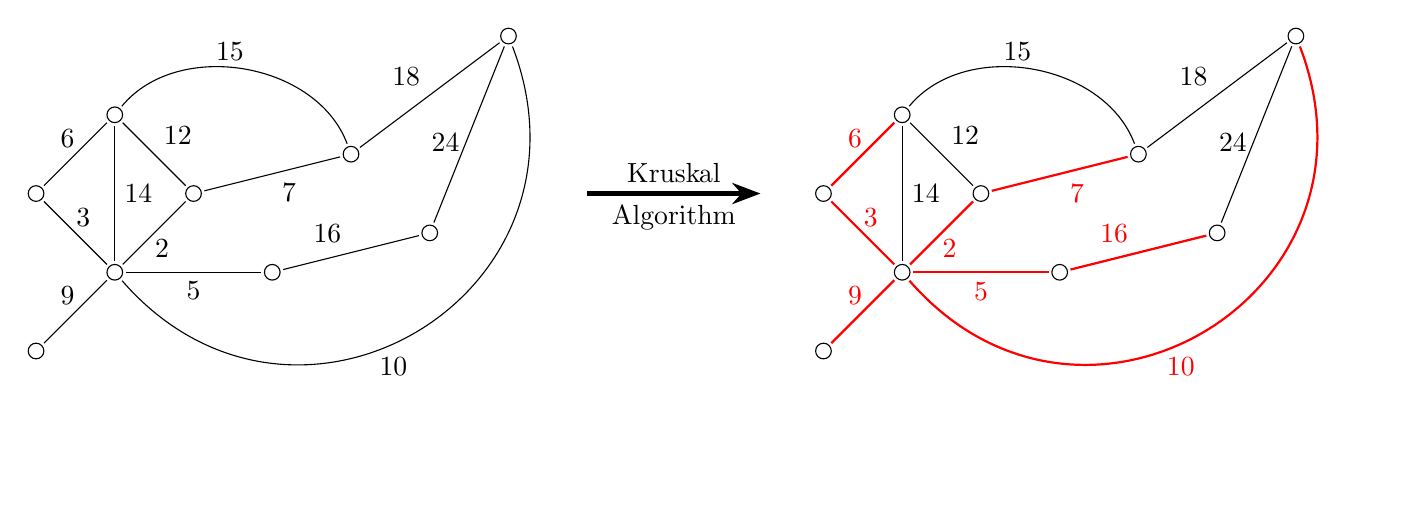
\begin{tikzpicture}[vertex/.style={circle, draw, fill=white, inner sep=2pt}]
		\begin{scope}[shift={(-5,0)}]
			\node[vertex] (1) at (0, 0) {};
			\node[vertex] (2) at (1, 1) {};
			\node[vertex] (3) at (1, -1) {};
			\node[vertex] (4) at (2, 0) {};
			\node[vertex] (5) at (4, 0.5) {};
			\node[vertex] (6) at (6, 2) {};
			\node[vertex] (7) at (5, -0.5) {};
			\node[vertex] (8) at (3, -1) {};
			\node[vertex] (9) at (0, -2) {};

			%    % Edges with weights (some edges have bends to avoid crossing)
			\draw[shorten >=1pt, shorten <=1pt] (1) -- (2) node[midway, xshift=-1mm,yshift=2mm] {6};
			\draw[shorten >=1pt, shorten <=1pt] (1) -- (3) node[midway, xshift=1mm,yshift=2mm] {3};
			\draw[shorten >=1pt, shorten <=1pt] (2) -- (3) node[midway, right] {14};
			\draw[shorten >=1pt, shorten <=1pt] (2) -- (4) node[midway, above right] {12};
			\draw[shorten >=1pt, shorten <=1pt] (3) -- (4) node[midway, xshift=1mm,yshift=-2mm] {2};
			\draw[shorten >=1pt, shorten <=1pt] (4) -- (5) node[midway, below right] {7};
			\draw[shorten >=1pt, shorten <=1pt] (2) to [bend left=60] (5) node[xshift=-1.5cm, yshift=1.2cm] {15};
			\draw[shorten >=1pt, shorten <=1pt] (5) -- (6) node[midway, above left] {18};
			\draw[shorten >=1pt, shorten <=1pt] (6) -- (7) node[midway, xshift=-3mm, yshift=-1mm] {24};
			\draw[shorten >=1pt, shorten <=1pt] (7) -- (8) node[midway, above left]{16};
			\draw[shorten >=1pt, shorten <=1pt] (3) -- (8) node[midway, below] {5};
			\draw[shorten >=1pt, shorten <=1pt] (3) to [bend right=80, looseness=1.5] (6) node[xshift=-1.5cm, yshift=-4.1cm] {10};
			\draw[shorten >=1pt, shorten <=1pt] (3) -- (9) node[midway, xshift=-1mm,yshift=2mm] {9};
		\end{scope}
		\draw[ultra thick, -Stealth] (2,0)  -- (4.2,0) node[midway, above] {Kruskal} node[midway, below] {Algorithm};
		\begin{scope}[shift={(5,0)}]
			\node[vertex] (1) at (0, 0) {};
			\node[vertex] (2) at (1, 1) {};
			\node[vertex] (3) at (1, -1) {};
			\node[vertex] (4) at (2, 0) {};
			\node[vertex] (5) at (4, 0.5) {};
			\node[vertex] (6) at (6, 2) {};
			\node[vertex] (7) at (5, -0.5) {};
			\node[vertex] (8) at (3, -1) {};
			\node[vertex] (9) at (0, -2) {};

			%    % Edges with weights (some edges have bends to avoid crossing)
			\draw[shorten >=1pt, shorten <=1pt, red, thick] (1) -- (2) node[midway, xshift=-1mm,yshift=2mm] {6};
			\draw[shorten >=1pt, shorten <=1pt, red, thick] (1) -- (3) node[midway, xshift=1mm,yshift=2mm] {3};
			\draw[shorten >=1pt, shorten <=1pt] (2) -- (3) node[midway, right] {14};
			\draw[shorten >=1pt, shorten <=1pt] (2) -- (4) node[midway, above right] {12};
			\draw[shorten >=1pt, shorten <=1pt, red, thick] (3) -- (4) node[midway, xshift=1mm,yshift=-2mm] {2};
			\draw[shorten >=1pt, shorten <=1pt, red, thick] (4) -- (5) node[midway, below right] {7};
			\draw[shorten >=1pt, shorten <=1pt] (2) to [bend left=60] (5) node[xshift=-1.5cm, yshift=1.2cm] {15};
			\draw[shorten >=1pt, shorten <=1pt] (5) -- (6) node[midway, above left] {18};
			\draw[shorten >=1pt, shorten <=1pt] (6) -- (7) node[midway, xshift=-3mm, yshift=-1mm] {24};
			\draw[shorten >=1pt, shorten <=1pt, red, thick] (7) -- (8) node[midway, above left]{16};
			\draw[shorten >=1pt, shorten <=1pt, red, thick] (3) -- (8) node[midway, below] {5};
			\draw[shorten >=1pt, shorten <=1pt, red, thick] (3) to [bend right=80, looseness=1.5] (6) node[xshift=-1.5cm, yshift=-4.1cm] {10};
			\draw[shorten >=1pt, shorten <=1pt, red, thick] (3) -- (9) node[midway, xshift=-1mm,yshift=2mm] {9};
		\end{scope}
	\end{tikzpicture}
\end{center}
The Kruskal algorithm uses a concept of component to find the minimum spanning tree.
\begin{Definition}{Component}{}
	In a graph $G=(V,E)$, a \emph{component} is a maximal subgraph $G'=(V',E')$ of $G$ such that \begin{enumerate}[label=(\arabic*)]
		\item $(V',E')$ is connected.
		\item $\forall\ v\notin V'$, there is no edge $e\in E$ such that $e$ connects $v$ to any vertex in $V'$.
	\end{enumerate}
\end{Definition}
In Kruskal algorithm we maintain a set of components each of them is a tree so basically we maintain a forest. And we find a safe edge which is always the least weight edge in the graph that connects two distinct components and add that edge to the collection of edges in the forest and update the components.

So the algorithm first sorts the edges in non-decreasing order of their weights. Then it initializes a forest $F$ with all the vertices in the graph and no edges. Then it iterates through the sorted edges and checks if the edge connects two distinct components. If it does, then it adds the edge to the forest and merges the two components. The algorithm stops when we have $n-1$ edges in the forest.
\begin{algorithm}[]
	\SetKwComment{Comment}{// }{}
	\caption{\textsc{Kruskal Algorithm}}
	\DontPrintSemicolon
	\KwIn{$G=(V,E)$, and weights of edges $W=\{w_e\in\bbZ_0\colon e\in E\}$}
	\KwOut{A minimum spanning tree $T\subseteq E$ of $G$}
	\Begin{
		\If{$G$ is not connected}{
			\Return{None}\Comment*{Use DFS or BFS}
		}
		$T\longleftarrow\emptyset$\;
		Sort the edges in $E$ in non-decreasing order of their weights so that $w(e_1)\leq w(e_2)\leq\cdots \leq w(e_m)$\;
		\For{$i=1,\dots, m$}{
			Let $e_i=(u,v)$\;
			\If{$T\cup\{e_i\}$ is acyclic}{
				$T\longleftarrow T\cup\{e_i\}$
			}
			\If{$|T|=|V|-1$}{
				\Return{$T$}\;
			}
		}
	}
\end{algorithm}
We have shown in \lmref{graphic-matroid} that the set of collection of acyclic sets in any graph is a matroid. Hence, here we are basically finding a base of the graphic matroid with minimum weight. The algorithm is exactly similar to the greedy algorithm for finding max-weight base of a matroid in \autoref{matroid-max-weight-base}. So you can use the similar arguments to show that the algorithm is correct and returns the minimum spanning tree of the graph.

Now in the algorithm the checking of $T\cup \{e_i\}$ is acyclic can be done by checking if both the end points are in same component or not. And if they are not then we need to combine those to components. But there comes a question:
\begin{question}{}
	What it means to give a component?
\end{question}
We will use some vertex to represent the component. We keep a pointer $v.\emph{parent}$ for each vertex which points to representative of component $v$ is in. Hence, we need a data structure that can do the following two operations efficiently:
\begin{itemize}[label=$\bullet$]
	\item \textsc{Find}$(u)$: Returns the component $u$ is in.
	\item \textsc{Union}$(u,v)$: Merges the components of $u$ and $v$ into a single component.
\end{itemize}
So we can use the updated algorithm to implement the Kruskal algorithm  using proper data structure:
\begin{algorithm}[]
	\SetKwComment{Comment}{// }{}
	\caption{\textsc{Kruskal Algorithm}}
	\DontPrintSemicolon
	\KwIn{$G=(V,E)$, and weights of edges $W=\{w_e\in\bbZ_0\colon e\in E\}$}
	\KwOut{A minimum spanning tree $T\subseteq E$ of $G$}
	\Begin{
		\If{$G$ is not connected}{
			\Return{None}\Comment*{Use DFS or BFS}
		}
		$T\longleftarrow\emptyset$\;
		Sort the edges in $E$ in non-decreasing order of their weights so that $w(e_1)\leq w(e_2)\leq\cdots \leq w(e_m)$\;
		\For{$i=1,\dots, m$}{
			Let $e_i=(u,v)$\;
			\If{$\textsc{Find}(u)\neq \textsc{Find}(v)$}{
				$T\longleftarrow T\cup\{e_i\}$\;
				\textsc{Union}$(u,v)$
			}
			\If{$|T|=|V|-1$}{
				\Return{$T$}\;
			}
		}
	}
\end{algorithm}
The Kruskal Algorithm calls $m$ times the \textsc{Find} operation and $n$ times the \textsc{Union} operation.
\section{Data Structure 1: Linear Array}
We create an $n$ length array $A$ which hold the parent pointer of each vertex. Initially for all vertices $A[v]=v$. So \textsc{Array-Find}$(u)$ will just return $A[u]$. Hence \textsc{Find} takes $O(1)$ time. For \textsc{Union}$(u,v)$ we use the following:
\begin{algorithm}[]
	\caption{\textsc{Array-Union}$(u,v)$}
	\DontPrintSemicolon
	\If{$A[u]\neq A[v]$}{
	\For{$i=1,\dots, n$}{
	\If{ $A[i]==A[v]$}{
	$A[i]\longleftarrow A[u]$\;
	}
	}
	}
\end{algorithm}
Therefore, \textsc{Array-Union}$(u,v)$ takes $O(n)$ time. Hence, the time complexity of the Kruskal algorithm using this data structure is $m\cdot O(1)+n\cdot O(n)=O(m+n^2)=O(n^2)$.
\section{Data Structure 2: Left Child Right Siblings Tree}
Using an array is not efficient enough.  One place we can optimize is if given the components is there a faster way to get the vertices in the component?  We can use the following tricks to optimize:
\begin{enumerate}[]
	\item For every representative of a component, store pointers to all vertices in that component.
	\item Change representative for the smaller component while doing \textsc{Union}$(u,v)$.
\end{enumerate}
\subsection{Construction}
So now every representative of a component we point to one vertex which is also in the component. And from that vertex we can iterate through all the vertices in that component. So basically we can immagine a 2 level tree where all the children point towards the root which is the representative of the component. The root points to one of the children take the left most child. And then all the other children points to the immediate right child of the root.
\begin{center}
	\usetikzlibrary{arrows.meta}
	\begin{tikzpicture}[vertex/.style={circle, draw, fill=white, inner sep=2pt}]
		\begin{scope}
			\node at (-2,0) {Initially we had:};
			\node[vertex] (1) at (0, 0) {};
			\node[vertex] (21) at (1, 0) {};
			\node[vertex] (22) at (1, -1) {};
			\node[vertex] (31) at (3, 0) {};
			\node[vertex] (32) at (2, -1) {};
			\node[vertex] (33) at (3, -1) {};
			\node[vertex] (34) at (4, -1) {};
			\node[vertex] (41) at (5, 0) {};
			\node[vertex] (42) at (5, -1) {};
			\path (1) edge [out=120, in=60, loop, min distance=0.4cm, -{Latex[length=1mm]}] (1);
			\path (21) edge [out=120, in=60, loop, min distance=0.4cm, -{Latex[length=1mm]}] (21);
			\path (31) edge [out=120, in=60, loop, min distance=0.4cm, -{Latex[length=1mm]}] (31);
			\path (41) edge [out=120, in=60, loop, min distance=0.4cm, -{Latex[length=1mm]}] (41);
			\draw[-{Latex[length=1mm]}] (22) -- (21);
			\draw[-{Latex[length=1mm]}] (42) -- (41);
			\foreach \x in {2,3,4} {
			\draw[-{Latex[length=1mm]}] (3\x) -- (31);
			}
			\path (31) edge[bend right=30, -{Latex[length=1mm]}, red] node[midway, left, font=\tiny] {Want} (32);
			\path (32) edge[-{Latex[length=1mm]}, red] node[midway, below, font=\tiny] {Want} (33);
		\end{scope}
		\begin{scope}[shift={(0,-2)}]
			\node at (-2,0) {Now we will do:};
			\node[vertex] (1) at (0, 0) {};
			\node[vertex] (21) at (1, 0) {};
			\node[vertex] (22) at (1, -1) {};
			\node[vertex] (31) at (3, 0) {};
			\node[vertex] (32) at (2, -1) {};
			\node[vertex] (33) at (3, -1) {};
			\node[vertex] (34) at (4, -1) {};
			\node[vertex] (41) at (5, 0) {};
			\node[vertex] (42) at (5, -1) {};
			\path (1) edge [out=120, in=60, loop, min distance=0.4cm, -{Latex[length=1mm]}] (1);
			\path (21) edge [out=120, in=60, loop, min distance=0.4cm, -{Latex[length=1mm]}] (21);
			\path (31) edge [out=120, in=60, loop, min distance=0.4cm, -{Latex[length=1mm]}] (31);
			\path (41) edge [out=120, in=60, loop, min distance=0.4cm, -{Latex[length=1mm]}] (41);
			\foreach \x in {2,4} {
					\draw[-right to,shorten <=1.15mm, shorten >=1.15mm] ($(\x2)+(0.02,0)$) -- ($(\x1)+(0.02,0)$);
					\draw[-right to,shorten <=1.15mm, shorten >=1.15mm] ($(\x1)+(-0.02,0)$) -- ($(\x2)+(-0.02,0)$);
				}
			\foreach \x in {3,4} {
			\draw[-{Latex[length=1mm]}] (3\x) -- (31);
			}
			\draw[-right to,shorten <=1mm, shorten >=1.2mm] ($(32)+(0.03,0)$) -- ($(31)+(0.03,0)$);
			\draw[-right to,shorten <=1mm, shorten >=1.2mm] ($(31)+(-0.03,0)$) -- ($(32)+(-0.03,0)$);
			\draw[-{Latex[length=1mm]}] (32) -- (33);
			\draw[-{Latex[length=1mm]}] (33) -- (34);
		\end{scope}
	\end{tikzpicture}
	\captionof{figure}{Left Child Right Sibling}
\end{center}
We can also store a variable to store the number of vertices in the component so that we can use it to compare the size of two components and then update for the smaller one. Therefore, the data structure now stores:
\begin{itemize}
	\item $v.\emph{parent}$ for each $v$ which points to the vertex representing the component $v$ is in.
	\item $v.\emph{size}$ for size of the component for each component representative $v$.
	\item $v.\emph{left}$ for the left most child for each component representative $v$.
	\item $v.\emph{right}$ for the immediate right sibling of $v$ for all vertices in a component which are not  representatives of the components.
\end{itemize}\parinf

This data structure is called Left Child Right Sibling. So in this data structure the \textsc{LCRS-Find}$(u)$ just returns the value of $u.\emph{parent}$. Hence, \textsc{LCRS-Find} takes $O(1)$ time.
\subsection{\textsc{LCRS-Union} Function}
For the \textsc{LCRS-Union} function we do the following
\begin{algorithm}[]
	\caption{\textsc{LCRS-Union}$(u,v)$}
	\DontPrintSemicolon
	$up\longleftarrow u.\emph{parent}$\; $vp\longleftarrow v.\emph{parent}$\;
	\If{$up\neq vp$}{
		\If{$up==u$}{
			$u.\emph{parent}\longleftarrow vp$\; $u.\emph{right}\longleftarrow vp.\emph{left}$\;
			$vp.\emph{left}\longleftarrow u$\; $vp.\emph{size}\longleftarrow vp.\emph{size}+1$\;
		}
		\ElseIf{$up.\emph{size}\leq vp.\emph{size}$}{
			$up.\emph{right}\longleftarrow u$\;
			$x\longleftarrow up$\;
			\While{$x.\emph{right}==None$}{
				$x.\emph{parent}\longleftarrow vp$, $x\longleftarrow x.\emph{right}$
			}
			$x.\emph{right}\longleftarrow vp.\emph{left}$\;
			$vp.\emph{left}\longleftarrow up.\emph{left}$\;
			$vp.\emph{left}\longleftarrow up$\;
			$vp.\emph{size}\longleftarrow vp.\emph{size}+\emph{up}.size$\;
		}
		\Else{
			$vp.\emph{right}\longleftarrow v$\;
			$x\longleftarrow vp$\;
			\While{$x.\emph{right}==None$}{
				$x.\emph{parent}\longleftarrow up$, $x\longleftarrow x.\emph{right}$
			}
			$x.\emph{right}\longleftarrow up.\emph{left}$\;
			$up.\emph{left}\longleftarrow vp.\emph{left}$\;
			$up.\emph{left}\longleftarrow vp$\;
			$up.\emph{size}\longleftarrow up.\emph{size}+\emph{vp}.size$\;
		}
	}
\end{algorithm}

Below we have shown how the \textsc{LCRS-Union} function works.
\begin{figure}[!h]
	\centering
	\begin{tikzpicture}[vertex/.style={circle, draw, fill=white, inner sep=2pt}]
		\begin{scope}
			\node at (-1,0) {(a)};
			\node[vertex] (21) at (0, 0) {};
			\node[vertex] (22) at (0, -1) {};
			\node[vertex] (31) at (2, 0) {};
			\node[vertex] (32) at (1, -1) {};
			\node[vertex] (33) at (2, -1) {};
			\node[vertex] (34) at (3, -1) {};
			\node[xshift=-0.3cm] at (0,0) {$up$};
			\node[xshift=0.3cm] at (2,0) {$vp$};
			\path (21) edge [out=120, in=60, loop, min distance=0.4cm, -{Latex[length=1mm]}] (21);
			\path (31) edge [out=120, in=60, loop, min distance=0.4cm, -{Latex[length=1mm]}] (31);
			\draw[-right to,shorten <=1.15mm, shorten >=1.15mm] ($(22)+(0.02,0)$) -- ($(21)+(0.02,0)$);
			\draw[-right to,shorten <=1.15mm, shorten >=1.15mm] ($(21)+(-0.02,0)$) -- ($(22)+(-0.02,0)$);
			\foreach \x in {3,4} {
			\draw[-{Latex[length=1mm]}] (3\x) -- (31);
			}
			\draw[-right to,shorten <=1mm, shorten >=1.2mm] ($(32)+(0.03,0)$) -- ($(31)+(0.03,0)$);
			\draw[-right to,shorten <=1mm, shorten >=1.2mm] ($(31)+(-0.03,0)$) -- ($(32)+(-0.03,0)$);
			\draw[-{Latex[length=1mm]}] (32) -- (33)  node[below]{$v$};
			\draw[-{Latex[length=1mm]}] (33) -- (34);
			\node at (22) [below] {$u$};
		\end{scope}
		\begin{scope}[shift={(5,0)}]
			\node at (0,0) {(b)};
			\node[vertex] (21) at (0, -1) {};
			\node[vertex] (22) at (1, -1) {};
			\node[vertex] (31) at (3, 0) {};
			\node[vertex] (32) at (2, -1) {};
			\node[vertex] (33) at (3, -1) {};
			\node[vertex] (34) at (4, -1) {};
			\node[below] at (0, -1) {$up$};
			\node[xshift=0.3cm] at (3,0) {$vp$};
			\draw[-{Latex[length=1mm]}] (22) -- (21);
			\path (21) edge[bend right=30, red, -{Latex[length=1mm]}] node [midway, below, font=\tiny, yshift=0.05cm]{\emph{right}} (22);
			\path (21) edge [out=120, in=60, loop, min distance=0.4cm, -{Latex[length=1mm]}] (21);
			\path (31) edge [out=120, in=60, loop, min distance=0.4cm, -{Latex[length=1mm]}] (31);
			\foreach \x in {3,4} {
			\draw[-{Latex[length=1mm]}] (3\x) -- (31);
			}
			\draw[-right to,shorten <=1mm, shorten >=1.2mm] ($(32)+(0.03,0)$) -- ($(31)+(0.03,0)$);
			\draw[-right to,shorten <=1mm, shorten >=1.2mm] ($(31)+(-0.03,0)$) -- ($(32)+(-0.03,0)$);
			\draw[-{Latex[length=1mm]}] (32) -- (33)  node[below]{$v$};
			\draw[-{Latex[length=1mm]}] (33) -- (34);
			\node at (22) [below] {$u$};
		\end{scope}
		\begin{scope}[shift={(11,0)}]
			\node at (0,0) {(c)};
			\node[vertex] (21) at (0, -1) {};
			\node[vertex] (22) at (1, -1) {};
			\node[vertex] (31) at (3, 0) {};
			\node[vertex] (32) at (2, -1) {};
			\node[vertex] (33) at (3, -1) {};
			\node[vertex] (34) at (4, -1) {};
			\node[below] at (0, -1) {$up$};
			\node[xshift=0.3cm] at (3,0) {$vp$};
			\path (21) edge[-{Latex[length=1mm]}] node [midway, below, font=\tiny, yshift=0.05cm]{\emph{right}} (22);
			\path (21) edge [bend left=15, -{Latex[length=1mm]}, red] node [midway, above, font=\tiny, rotate=13,yshift=-0.05cm] {\emph{parent}} (31);
			\path (22) edge [-{Latex[length=1mm]}, red] node [midway, above, font=\tiny, rotate=22, xshift=-0.3cm, yshift=-0.09cm] {\emph{parent}} (31);
			\path (31) edge [out=120, in=60, loop, min distance=0.4cm, -{Latex[length=1mm]}] (31);
			\draw[-{Latex[length=1mm]}] (21) -- (22);
			\foreach \x in {3,4} {
			\draw[-{Latex[length=1mm]}] (3\x) -- (31);
			}
			\draw[-right to,shorten <=1mm, shorten >=1.2mm] ($(32)+(0.03,0)$) -- ($(31)+(0.03,0)$);
			\draw[-right to,shorten <=1mm, shorten >=1.2mm] ($(31)+(-0.03,0)$) -- ($(32)+(-0.03,0)$);
			\draw[-{Latex[length=1mm]}] (32) -- (33)  node[below]{$v$};
			\draw[-{Latex[length=1mm]}] (33) -- (34);
			\node at (22) [below] {$u$};
		\end{scope}
		\begin{scope}[shift={(-1,-3)}]
			\node at (0,0) {(d)};
			\node[vertex] (21) at (0, -1) {};
			\node[vertex] (22) at (1, -1) {};
			\node[vertex] (31) at (3, 0) {};
			\node[vertex] (32) at (2, -1) {};
			\node[vertex] (33) at (3, -1) {};
			\node[vertex] (34) at (4, -1) {};
			\node[below] at (0, -1) {$up$};
			\node[xshift=0.3cm] at (3,0) {$vp$};
			\path (21) edge[-{Latex[length=1mm]}] node [midway, below, font=\tiny, yshift=0.05cm]{\emph{right}} (22);
			\path (21) edge [bend left=15, -{Latex[length=1mm]}] node [midway, above, font=\tiny, rotate=13,yshift=-0.05cm] {\emph{parent}} (31);
			\path (22) edge [-{Latex[length=1mm]}] node [midway, above, font=\tiny, rotate=22, xshift=-0.3cm, yshift=-0.09cm] {\emph{parent}} (31);
			\draw[-{Latex[length=1mm]},red] (22) -- node [midway, below, font=\tiny, yshift=0.05cm]{\emph{right}} (32);
			\path (31) edge [out=120, in=60, loop, min distance=0.4cm, -{Latex[length=1mm]}] (31);
			\draw[-{Latex[length=1mm]}] (21) -- (22);
			\foreach \x in {3,4} {
			\draw[-{Latex[length=1mm]}] (3\x) -- (31);
			}
			\draw[-right to,shorten <=1mm, shorten >=1.2mm] ($(32)+(0.03,0)$) -- ($(31)+(0.03,0)$);
			\draw[-right to,shorten <=1mm, shorten >=1.2mm] ($(31)+(-0.03,0)$) -- ($(32)+(-0.03,0)$);
			\draw[-{Latex[length=1mm]}] (32) -- (33)  node[below]{$v$};
			\draw[-{Latex[length=1mm]}] (33) -- (34);
			\node at (22) [below] {$u$};
		\end{scope}
		\begin{scope}[shift={(5,-3)}]
			\node at (0,0) {(e)};
			\node[vertex] (21) at (0, -1) {};
			\node[vertex] (22) at (1, -1) {};
			\node[vertex] (31) at (3, 0) {};
			\node[vertex] (32) at (2, -1) {};
			\node[vertex] (33) at (3, -1) {};
			\node[vertex] (34) at (4, -1) {};
			\node[below] at (0, -1) {$up$};
			\node[xshift=0.3cm] at (3,0) {$vp$};
			\path (21) edge[-{Latex[length=1mm]}]  (22);
			\path (22) edge [-{Latex[length=1mm]}]  (31);
			\draw[-{Latex[length=1mm]}] (22) --  (32);
			\path (31) edge [out=120, in=60, loop, min distance=0.4cm, -{Latex[length=1mm]}] (31);
			\draw[-{Latex[length=1mm]}] (21) -- (22);
			\foreach \x in {3,4} {
			\draw[-{Latex[length=1mm]}] (3\x) -- (31);
			}
			\draw[-{Latex[length=1mm]}] (32) -- (31);
			\draw[-{Latex[length=1mm]}] (32) -- (33)  node[below]{$v$};
			\draw[-{Latex[length=1mm]}] (33) -- (34);
			\draw[-{Latex[length=1mm]}] (21) -- (31);
			\node at (22) [below] {$u$};
			\path (31) edge [bend right=15, -{Latex[length=1mm]}, red] node [midway, above, font=\tiny, rotate=13,yshift=-0.05cm] {\emph{left}} (21);
		\end{scope}
		\begin{scope}[shift={(11,-3)}]
			\node at (0,0) {(f)};
			\node[vertex] (21) at (0, -1) {};
			\node[vertex] (22) at (1, -1) {};
			\node[vertex] (31) at (3, 0) {};
			\node[vertex] (32) at (2, -1) {};
			\node[vertex] (33) at (3, -1) {};
			\node[vertex] (34) at (4, -1) {};
			\path (21) edge[-{Latex[length=1mm]}]  (22);
			\path (22) edge [-{Latex[length=1mm]}]  (31);
			\draw[-{Latex[length=1mm]}] (22) --  (32);
			\path (31) edge [out=120, in=60, loop, min distance=0.4cm, -{Latex[length=1mm]}] (31);
			\draw[-{Latex[length=1mm]}] (21) -- (22);
			\foreach \x in {3,4} {
			\draw[-{Latex[length=1mm]}] (3\x) -- (31);
			}
			\draw[-{Latex[length=1mm]}] (32) -- (31);
			\draw[-{Latex[length=1mm]}] (32) -- (33)  node[below]{$v$};
			\draw[-{Latex[length=1mm]}] (33) -- (34);
			\node at (22) [below] {$u$};
			\draw[-right to,shorten <=1 mm, shorten >=1.5mm] ($(21)+(0.03,0.02)$) -- ($(31)+(0.03,0.02)$);
			\draw[-right to,shorten <=1mm, shorten >=1.2mm] ($(31)+(-0.03,0.05)$) -- ($(21)+(-0.03,0.05)$);
		\end{scope}
	\end{tikzpicture}
	\caption{A run of \textsc{LCRS-Union}$(u,v)$}
\end{figure}
This way we can unite two components and update the corresponding component representative in the vertices of the smaller component. In the next section we will analyze the amortized time complexity of the \textsc{LCRS-Union} function
\subsection{Amortized analysis of \textsc{LCRS-Union}}
\begin{lemma}{}{}
	For any vertex $v\in V$, $v.\emph{parent}$ can change at most $O(\log n)$ times.
\end{lemma}
\begin{proof}
	Initially size of $v$'s component is $1$. Each time $v.\emph{parent}$ is changed the size of the component $v$ is in becomes at least double. Therefore, at most $O(\log n)$ times $v.\emph{parent}$ can change.
\end{proof}\parinn

Now since there are $n$ vertices at most $O(n\log n)$ times change of \emph{parent} for any vertex happens. Now change of \emph{parent} for any vertex happens only in \textsc{LCRS-Union} function. Total time taken by all the \textsc{LCRS-Union} operations is $O(n\log n)$ time. Since \textsc{LCRS-Union} was called $n$ times the amortized cost of \textsc{LCRS-Union} is $O(\log n)$.
\subsection{Time Complexity Analysis of Kruskal}
We have shown above that \textsc{LCRS-Find} takes $O(1)$ time and amortized cost of \textsc{LCRS-Union} is $O(\log n)$. Since \textsc{LCRS-Find} is called $m$ times and \textsc{LCRS-Union} is called $n$ times the total run time of Kruskal Algorithm using the Left Child Right Sibling data structure is $O(m+n\log n)$.
\section{Data Structure 3: Union Find}
We will now give up on the idea of height $1$ trees to optimize more. Representative of a component is still vertex at root, but we will do the following: changes:
\begin{itemize}
	\item \textsc{Union} just changes parent pointers of root nodes, but it takes $O(1)$.
	\item Instead of size, we will maintain a variable \emph{rank} of a component roughly which can be thought of as height of the component.
	\item For \textsc{Union} root of smaller rank will be changed to point to root of the component of larger rank.
	\item The \textsc{Find} operation does something called path compression which we will explain later.
\end{itemize}
To implement this data structure we will use a tree for each component and every node has a \emph{parent} pointer. And there we will use the \textsc{Find} and \textsc{Union} operations.

Our goal is to run Kruskal algorithm in almost $O(n+m)$ time. More precisely $O((n+m)\log^* n)$ time where $\log ^*n$ is the number of times we need to compose $\log $ on $n$ to get $1$.
\subsection{\textsc{Find} Operation}
The \textsc{Find} operation does something called path compression i.e. for any vertex $v\in V$, if \textsc{Find}$(v)$ is called then it starts from $v$ changes it's parent to the root of the component $v$ is in and then it moves to its parent and changes his parent to be the root and move to his parent and keep on doing like that till it reaches the root. In other words in path from the root to $v$, for every vertex in that path the \textsc{Find} operation changes the \emph{parent} pointer to the root.
\begin{center}
	\usetikzlibrary{arrows.meta}
	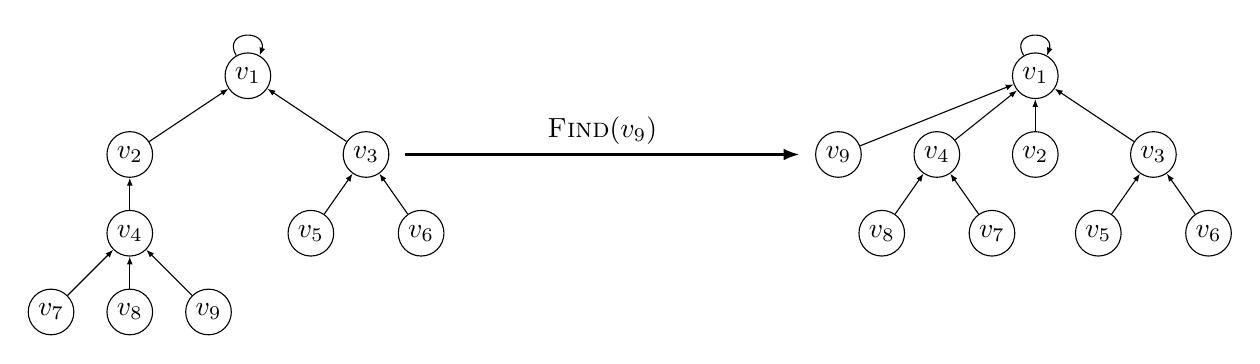
\begin{tikzpicture}[vertex/.style={circle, draw, fill=white, inner sep=2pt}]
		\begin{scope}
			\node[vertex] (1) at (0, 0) {$v_1$};
			\node[vertex] (22) at (1.5, -1) {$v_3$};
			\node[vertex] (21) at (-1.5, -1) {$v_2$};
			\node[vertex] (31) at (-1.5, -2) {$v_4$};
			\node[vertex] (32) at (0.8, -2) {$v_5$};
			\node[vertex] (33) at (2.2, -2) {$v_6$};
			\node[vertex] (41) at (-0.5, -3) {$v_9$};
			\node[vertex] (42) at (-1.5, -3) {$v_8$};
			\node[vertex] (43) at (-2.5, -3) {$v_7$};
			\path (1) edge [out=120, in=60, loop, min distance=0.4cm, -{Latex[length=1mm]}] (1);
			\draw[-{Latex[length=1mm]}] (21) -- (1);
			\draw[-{Latex[length=1mm]}] (22) -- (1);
			\draw[-{Latex[length=1mm]}] (31) -- (21);
			\draw[-{Latex[length=1mm]}] (32) -- (22);
			\draw[-{Latex[length=1mm]}] (33) -- (22);
			\draw[-{Latex[length=1mm]}] (41) -- (31);
			\draw[-{Latex[length=1mm]}] (42) -- (31);
			\draw[-{Latex[length=1mm]}] (43) -- (31);
		\end{scope}
		\begin{scope}[shift={(10,0)}]
			\node[vertex] (A1) at (0, 0) {$v_1$};
			\node[vertex] (A22) at (1.5, -1) {$v_3$};
			\node[vertex] (A21) at (0, -1) {$v_2$};
			\node[vertex] (A31) at (-1.25, -1) {$v_4$};
			\node[vertex] (A32) at (0.8, -2) {$v_5$};
			\node[vertex] (A33) at (2.2, -2) {$v_6$};
			\node[vertex] (A41) at (-0.55, -2) {$v_7$};
			\node[vertex] (A42) at (-1.95, -2) {$v_8$};
			\node[vertex] (A43) at (-2.5, -1) {$v_9$};
			\path (A1) edge [out=120, in=60, loop, min distance=0.4cm, -{Latex[length=1mm]}] (A1);
			\draw[-{Latex[length=1mm]}] (A21) -- (A1);
			\draw[-{Latex[length=1mm]}] (A22) -- (A1);
			\draw[-{Latex[length=1mm]}] (A31) -- (A1);
			\draw[-{Latex[length=1mm]}] (A32) -- (A22);
			\draw[-{Latex[length=1mm]}] (A33) -- (A22);
			\draw[-{Latex[length=1mm]}] (A41) -- (A31);
			\draw[-{Latex[length=1mm]}] (A42) -- (A31);
			\draw[-{Latex[length=1mm]}] (A43) -- (A1);
		\end{scope}
		\draw[thick, -{Latex[length=2mm]}, shorten <=2mm, shorten >= 2mm] (22) -- node[midway, above] {\textsc{Find}$(v_9)$} (A43);
	\end{tikzpicture}
	\captionof{figure}{Path compression during \textsc{Find}$(v_9)$ operation}
\end{center}
Here is the pseudocode of the \textsc{Find} operation below:
\begin{algorithm}[]
	\caption{\textsc{Find}$(v)$}
	\DontPrintSemicolon
	\If{$v.\emph{parent}\neq v$}{
		$v.\emph{parent}\longleftarrow \textsc{Find}(v.\emph{parent})$\;
	}
	\Return{$v.\emph{parent}$}
\end{algorithm}We will not discuss the amortized cost of this operation. Instead, we will do it in \autoref{analysis-union-find}.
\subsection{\textsc{Union} Operation}
For the \textsc{Union} operation we change the root of smaller rank to point to the root of the component of larger rank. So for the \textsc{Union}$(u,v)$ operation we assume that $u$, $v$ are the roots of their respective components. 
\begin{algorithm}[]
	\caption{\textsc{Union}$(u,v)$}
	\SetKwComment{Comment}{// }{}
	\DontPrintSemicolon
	\If{$u.\emph{rank}>v.\emph{rank}$}{
		$v.\emph{parent}\longleftarrow v$\;
	}
	\ElseIf{$v.\emph{rank}>u.\emph{rank}$}{
		$u.\emph{parent}\longleftarrow v$\;
	}
	\Else{
		$v.\emph{parent}\longleftarrow u$\;
		$v.\emph{rank}\longleftarrow v.\emph{rank}+1$
	}
\end{algorithm}
Since in \textsc{Union}$(u,v)$ we assume $u,v$ are component representatives before using \textsc{Union}$(u,v)$ we use \textsc{Find} on $u$ and $v$ to get the roots of their components, and then we apply \textsc{Union} on the roots. Hence, \textsc{Union}$(u,v)$ takes $O(1)$ time.
\subsection{Analyzing the Union-Find Data-Structure}\label{analysis-union-find}
We call a node in the union-find data-structure a \emph{leader} if it is the root of the (reversed) tree.
\begin{lemma}{}{}
	Once a node stop being a {leader} (i.e. the node in top of a tree). It can never become a leader again.
\end{lemma}
\begin{proof}
	A node $x$ stops being a {leader} only because of the \prb{Union} operation which made $x$ child of a node $y$ which is a {leader} of a tree. From this point on, the only operation that might change the parent pointer of $x$ is the \prb{Find} operation which traverses through $x$. Since path-compression only change the parent pointer of $x$ to point to some other node $y$. Therefore, the parent pointer of $x$ will never become equal to itself i.e. $x$ can never be a {leader} again. Hence, once $x$ stops being a {leader} it can never be a {leader} again.
\end{proof}
\begin{lemma}{}{}
	Once a node stop being a leader then its rank is fixed.
\end{lemma}
\begin{proof}
	The rank of a node changes only by a \prb{Union} operation. But the \prb{Union} operation only changes the rank of nodes that are {leader} after the operation is done. Therefore, once a node stops being a {leader} it's rank will not being changed by a \prb{Union} operation. Hence, once a node stop being a leader then its rank is fixed.
\end{proof}
\begin{lemma}{}{}
	Ranks are monotonically increasing in the reversed trees, as we travel from a node to
	the root of the tree.
\end{lemma}
\begin{proof}
	To show that the ranks are monotonically increasing  it suffices to prove that for all edge $u\to v$ in the data structure we have $\Rank(u)<\Rank(v)$.
\end{proof}

\begin{lemma}{}{}
	When a node gets rank $k$ than there are at least $\geq 2^k$ elements in its subtree.
\end{lemma}
\begin{corolary}{}{}
	For all vertices $v$, $v.rank\leq \lt\lfloor \log n\rt\rfloor$
\end{corolary}
\begin{corolary}{}{}
	Height of any tree $\leq \lt\lfloor\log _2n\rt\rfloor$
\end{corolary}
\begin{lemma}{}{}
	The number of nodes that get assigned rank $k$ throughout the execution of the Union-Find data-structure is at most $\frac{n}{2^k}$.
\end{lemma}
Define $N(r)=\#$vertices with rank at least $k$. Then by the above lemma we have $N(r)\leq \frac{n}{2^k}$.
\begin{lemma}{}{}
	The time to perform a single find operation when we perform union by rank and path
	compression is $O(\log n)$ time.
\end{lemma}
We will show that we can do much better. In fact, we will show that for $m$ operations over $n$ elements the overall running time is $O((n+m)\log ^*n)$

\begin{lemma}{}{}
	During a single $\prb{Find}(x)$ operation, the number of jumps between blocks along the search path is $O(\log^*n)$.
\end{lemma}
\begin{lemma}{}{}
	At most $|\emph{Block}(i)|\leq \emph{Tower}(i)$ many \prb{Find} operations can pass through an element $x$ which is in the $i^{th}$ block (i.e. $\prb{index}_B(x)=i$) before $x.\emph{parent}$ is no longer in the $i^{th}$ block. That is $\prb{index}_B(x.\emph{parent})>i$.
\end{lemma}

\begin{lemma}{}{}
	There are at most $\frac{n}{\emph{Tower}(i)}$ nodes that have ranks in the $i^{th}$ block throughout the algorithm execution.
\end{lemma}

\begin{lemma}{}{}
	The number of internal jumps performed, inside the $i^{th}$ block, during the lifetime of \prb{Union-Find} data structure is $O(n)$.
\end{lemma}

\begin{Theorem}{}{}
	The number of internal jumps performed by the \prb{Union-Find} data structure overall $O(n\log^*n)$.
\end{Theorem}
\begin{Theorem}{}{}
	The overall time spent on $m$ \prb{Find} operations, throughout the lifetime of a Union-Find data structure defined over $n$ elements is $O((n+m)\log^*n)$.
\end{Theorem}
%\chapter{Red Black Tree}
A red-black tree is a special type of binary search tree with one extra bit of storage per node, its color which can be either red or black. Also, we keep the tree approximately balanced by enforcing some properties on the tree.
\begin{definition}{Perfect Binary Tree}{}
	It is a Binary Tree in which every internal node has exactly two children and all leaves are at the same level.
\end{definition}
\begin{Lemma}{}{}
	Every perfect binary tree with $k$ leaves has $2k-1$  nodes (i.e. $k-1$ internal nodes).
\end{Lemma}
\begin{definition}{Red Black Tree}{}
	\begin{minipage}{0.5\textwidth}
		A red-black tree is a binary tree with the following properties:
		\begin{itemize}
			\item Every internal node is key/NIL node. Every leaf is a ``NIL'' node.
			\item Each node (NIL and key) is colored either red or black.
			\item  Root and NIL nodes are always black.
			\item Any child of a red node is black.
			\item The path from root to any leaf has the same number of black nodes.
		\end{itemize}
	\end{minipage}\hfill
	\begin{minipage}{0.49\textwidth}
		\centering
		\usetikzlibrary{trees,arrows,positioning, calc}
		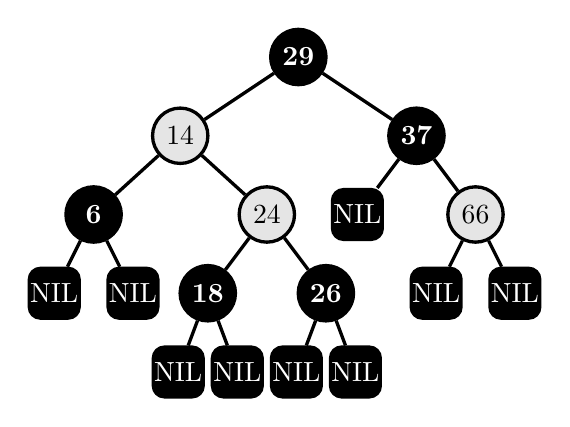
\begin{tikzpicture}[very thick,
				level/.style={sibling distance=30mm/#1},
				level distance=10mm,
				redVertex/.style={draw,fill=black!10!white,circle,minimum size=20pt,inner sep=0pt},
				blackVertex/.style={draw,fill=black,   circle,minimum size=20pt,inner sep=0pt, text=white, font=\bfseries},
				nil/.style={draw,fill=black,rectangle,rounded corners, minimum size=18pt,inner sep=0pt, text=white}]
			\node [blackVertex] (r){29}
			child {
					node[redVertex] {14}
					child [sibling distance=22mm] {
							node[blackVertex] {6}
							child {node [nil] {NIL}}
							child {node [nil] {NIL}}
						}
					child [sibling distance=22mm] {
							node [redVertex] {24}
							child [sibling distance=15mm] {
									node [blackVertex] {18}
									child {node [nil] {NIL}}
									child {node [nil] {NIL}}
								}
							child [sibling distance=15mm] {
									node [blackVertex] {26}
									child {node [nil] {NIL}}
									child {node [nil] {NIL}}
								}
						}
				}
			child {
					node[blackVertex] {37}
					child {node [nil] {NIL}}
					child {
							node [redVertex] {66}
							child {node [nil] {NIL}}
							child { node [nil] {NIL}}
						}
				};
		\end{tikzpicture}
		\captionof{figure}{A Red Black Tree}
		\label{fig:red-black-tree}
	\end{minipage}
\end{definition}

We call the number of black nodes on any simple path from  but not including a node $x$ down to a leaf the \emph{black-height} of the node, denoted by $bh(x)$. We generally confine our interest to the internal nodes of a red-black tree, since they hold the key values.
\begin{Lemma}{}{}
	A Red-Black Tree with $n$ internal nodes or key nodes has height at most $O(\log n)$.
\end{Lemma}
\begin{proof}
	We will first show that for any subtree rooted at node $x$ contains at least $2^{bh(x)}-1$ internal nodes. We will show this using induction on the height of the tree. For the base case let height of $x$ is $0$. Then $x$ must be a leaf. Therefore, the subtree rooted at $x$ has at least $bh(x)=0$. Hence, $2^{bh(x)}-1=2^0-1=0$  nodes which is true. For inductive step let $x$ has some positive height, and it is an internal node of the R-B Tree. Now $x$ has two children. Hence, each child has black-height either $bh(x)$ or $bh(x)-1$. By inductive hypothesis, the subtrees rooted at the children of $x$ have at least $2^{bh(x)-1}-1$ internal nodes. Thus, subtree rooted at $x$ has at least $2^{bh(x)-1}-1+2^{bh(x)-1}-1+1=2^{bh(x)}-1$ internal nodes.

	Now if the R-B tree has height $h$. Then any path from the root to a leaf at least half the nodes including the root must be black. So $bh(\emph{root})\geq \frac{h}2$. Thus, $n\geq 2^{\frac{h}2}-1\implies h\leq 2\log(n+1)$. Hence, we have the lemma.
\end{proof}
\nt{
	\begin{minipage}{0.3\textwidth}
		\centering
		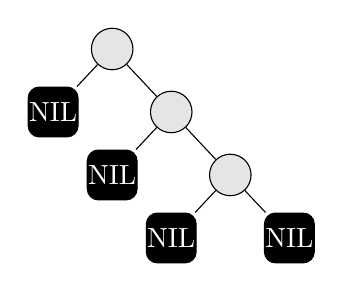
\begin{tikzpicture}[
				level distance=8mm,
				vertex/.style={draw,fill=black!10!white,circle,minimum size=15pt,inner sep=0pt},
				nil/.style={draw,fill=black,rectangle,rounded corners, minimum size=18pt,inner sep=0pt, text=white}
			]
			\node[vertex] (a) {}
			child { node [nil] {NIL} }
			child {
					node [vertex] (b) {}
					child { node [nil] {NIL} }
					child {
							node [vertex] (c) {}
							child { node [nil] {NIL} }
							child { node [nil] {NIL} }
						}
				};
		\end{tikzpicture}
	\end{minipage}\hfill
	\begin{minipage}{0.69\textwidth}
		Not all trees can be colored in a way that satisfies the properties of a red-black tree. Consider the following tree:\parinn

		In this example the root has to be black. The other two internal nodes can not be black since otherwise the path from the leaf of the root to root has only 2 black nodes but in the path from bottom most leaf to root will have 3. Then those two internal nodes has to be red. But that violates the property that a red node can not have a red child. Hence, this tree can not be colored in a way that satisfies the properties of a red-black tree.
	\end{minipage}
}

%\chapter{Max Flow Min Cut}
%\chapter{Randomized Algorithm}
Here we will study randomized algorithm for tow basic problems. Later we will discuss other randomized algorithms too in the next chapters. We will also try to derandomize an algorithm in the next chapter.
\section{Estimated Binary Search Tree Height}
In this section we will calculate the expected height of a tree obtained by constructing a binary tree by picking elements uniformly at random from a given array. For this we have the following simple \prb{Intersection Algorithm}

\begin{algorithm}
\KwIn{Array $A$ of $n$ elements of $[n]$ in any order.}
\KwOut{Construct a binary tree from $A$}
\DontPrintSemicolon\Begin{
$S\longleftarrow A$\;
$T\longleftarrow \emptyset$\;
\While{$S\neq\emptyset$}{
$u\longleftarrow\prb{Extract}(S)$\;
Insert each element at the appropriate leaf of $T$\;
}
\Return{$T$}
}
\caption{Simple Intersection Algorithm}
\end{algorithm}

\begin{question}{}{}
	What is the expected height of the tree obtained by this \prb{Simple Intersection Algorithm} assuming sequence of keys is uniformly random permutation of $[n]$.
\end{question}

Suppose $X_n$ be the random variable for the height of the tree obtained by the algorithm running on any permutation of $[n]$. Let $R_n$ be the random variable for the root of the tree obtained by the algorithm. Now consider the random variable $Y_n$ defined as $Y_n=2^{X_n}$. Then, if we know $R_n=i$ we have  $$X_n=1+\max\{\text{Height of left subtree, Height of right subtree}\}=1+\max\{X_{i-1}+X_{n-i}\}\implies Y_n=2\max\{Y_{n-1},Y_{n-i}\}$$Now for the case of $n=1$ $Y_1=1$  since there is only one element and for the convenience we define $Y_0=0$. Now consider the following indicator random variable $Z_{n,i}$ where $$Z_{n,i}=\begin{cases}
	1 & \text{if $i$ is first element}\\ 0 & \text{otherwise}
\end{cases}$$So basically $Z_{n,i}=\mathbbm{1}{\{R_n=i\}}$. Now if $i$ is the first element then $i$ the root of the tree obtained by the algorithm. Therefore we have \begin{align*}
Y_n &=\sum\limits_{i=1}^n Z_{n,i}\lt(1+\max\{Y_{i-1},Y_{n-i}\}\rt)\\
& \leq 2\sum\limits_{i=1}^nZ_{n,i}(Y_{i-1}+Y_{n-i}) & [\text{Using \lmref{softmax}}]
\end{align*}

\begin{lemma}{Soft Max}{softmax}
	For any $a,b\in \bbR$, $$\max\{a,b\}\leq \log (2^a+2^b)$$
\end{lemma}


Therefore, we have \begin{align*}
	\bbE[Y_n] & \leq 2\sum\limits_{i=1}^n\bbE\Big[Z_{n,i}(Y_{i-1}+ Y_{n-i})\Big]\\
	& = 2\sum\limits_{i=1}^n\bbE[Z_{n,i}]\bbE[Y_{i-1}+ Y_{n-i}]\\
	& = \frac2n\sum_{i=1}^n (\bbE[Y_{i-1}]+\bbE[Y_{n-i}])=\frac4n\sum_{i=0}^{n-1}\bbE[Y_i]
\end{align*}

Now to compute $\bbE[Y_n]$ we use the following lemma
\begin{lemma}{}{}
	$\dps{\bbE[Y_n]\leq\frac14\binom{n+3}{3}}$
\end{lemma}
\begin{proof}
	We will prove this using induction on $n$. The base case is true for $n=0$. Suppose this is true for $0,\dots, n-1$. $$	\bbE[Y_n]\leq \frac4n\sum_{i=0}^{n-1}\bbE[Y_i]\leq \frac1n\sum_{i=0}^{n-1}\binom{i+3}{3}= \frac1n\binom{n+3}{4}= \frac1n\frac{(n+3)!}{4!(n-1)!}= \frac14\binom{n+3}{3}$$Hence by  mathematical induction  this is true for all $n$. 
\end{proof}

Hence, by the lemma we have $\bbE[Y_n]\leq\frac14\binom{n+3}{3}=O(n^3)$. Now by Jensen Inequality we have $$\bbE[Y_n]=\bbE[2^{X_n}]\geq 2^{\bbE[X_n]}$$Therefore $\bbE[X_n]\leq O(\log n)$. Therefore, the expected height of a binary search tree is $O(\log n)$. 
\section{Solving 2-\prb{SAT}}
In this section we will discuss a randomized algorithm for deciding if a $n$-variate 2-SAT boolean formula is satisfiable or not.

\begin{algoprob}
	\problemtitle{2-SAT}
	\probleminput{2-SAT formula $\vph$ consisting of $n$ variables.}
	\problemquestion{Given $n$-variate 2-SAT boolean formula determine if $\vph$ is satisfiable.}
\end{algoprob}\parinf

Here we give a simple randomized algorithm for solving the 2-SAT problem:\parinn\newpage

\begin{algorithm}
\KwIn{$n$ variate 2-SAT formula $\vph$}
\KwOut{Decide if $\vph$ is satisfiable or not}
\DontPrintSemicolon
\Begin{
$\forall\ i\in[n]$, Set $x_i=0$\;
\While{$\exs$ clause $C$ that is not satisfied}{
Let $x_i$ and $x_j$ be variables in $C$\;
Pick from $\{x_i,x_j\}$ with equal probability and flip the assignment for that variable.
}
\Return{$x$}
}
\caption{2-SAT Randomized Algorithm}
\end{algorithm}

Now if the algorithm terminates it terminates with a satisfying assignment. For now assume that $\vph$ is satisfiable. We will deal with the case that $\vph$ is not satisfiable later. 

Now since there are $n$ variables there can be at most $O(n^2)$ many clauses can be in the formula. Therefore, for each step of the while loop to occur it can at most take $O(n^2)$ time to find a clause which is not satisfied.

Let $S$ represents the set of satisfying assignments for $\vph$. Let at $j^{th}$ iteration let $A_j$ denote the current assignment of the variables. Let $X_j$ be the random variable which denotes maximum number of variables of $A_j$ that matches with some satisfying assignment of $S$ i.e. $$X_j=\max\{n-|x-A_j|\colon x\in S\}$$At any step if $X_j=n$ then the algorithm terminates since the algorithm has found a satisfying assignment. Now starting with $X_j<n$ we consider how $X_j$ evolves over time and how long it takes before $X_j$ reaches $n$.

Now at each step we pick a clause which is unsatisfied. So we know $A_j$ and all assignments of $S$ disagree on the value of at least one variable of this clause. If all the assignments in $S$ disagree with $A_j$ on both variables changing either one will increase $X_j$. If there are assignments in $S$ which disagree on the value of one of the two variables then with probability $\frac12$ we choose that variable and increase $X_j$ by 1 and with probability $\frac12$ we choose the other variable and decrease $X_j$ by $1$.

Therefore, $X_j$ behaves like a random walk on a line starting from $0$ which denotes the worst possible case and ends once it reaches at $n$ where at any nonzero point it goes up or down by 1 with probability $\frac12$. This is a Markov Chain. We want to calculate how many steps does it take on average for $X_j$ to stumble all the way up to $n$. Before that we first properly define our Markov Chain.

The Markov Chain consists states from $0 $ to $n$. Where from 0 it goes to 1 with probability 1 and from $n$ it always stays at $n$. And for any other state $i$ it goes to $i+1$ with probability $\frac12$ and goes to $i-1$ with probability $\frac12$. Now let $$T(k)=\text{Expected time to walk from $k$ to $n$}$$ Then we have $$T(n)=0,\qquad T(0)=T(1)+1, \qquad\forall\ i\in [n-1],\ T(i)=\frac{T(i-1)}{2}+\frac{T(i+1)}2+1$$Then we have $n$ unknowns and $n$ equations in the above system. Therefore, on average at most $O(n^2)$ steps needed to find a solution.

Now at first we said we are assuming we are dealing with the case of there exists a solution. 
\begin{question}{}{}
	How to deal with the issue of no solution?
\end{question}
In this case we will run for more number of iterations before we give up since when we give up we me might just not have found the solution. So we will run the algorithm for $100n^2$ steps. And if no solution was found then we will give up. 

We first of all divide the execution of the algorithm into segments of $2n^2$ steps each. We will calculate the failure case of each segment. If the 2-SAT formula has no solution then the algorithm gives correct output. Suppose it has a solution. Then by Markov's Inequality the probability of number of steps needed to find the solution is greater than the expected number of steps needed to find a solution is at most $\frac12$. Now after total $100n^2$ steps the probability none of the segments found a solution is $2^{-50}$.
%\chapter{Derandomization}
In this section we will see a derandomization technique called Conditional Expectation. With this technique we will show derandomization of some randomized algorithms in the following sections.
\section{Conditional Expectation}
Let $\sA$ be a randomized algorithm which is successful with probability at least $\frac23$. Suppose $\sA$ uses $m$ random bits and suppose the random bits are $R_1,\dots , R_m$. Then we have $$\underset{R_1,\dots, R_m}{\bbP}[\sA(x,R_1,\dots, R_m)=\text{Correct}]\geq \frac23$$We want to derandomize $\sA$.

Now think of $\sA$ as a binary tree which, given $x$, branches on the sampled value of each random bit $R_i$ where it goes to left child if the random bit takes value $0$ and goes to right child if the random bit takes value $1$. Every path in this tree from root to leaf corresponds to different possible random strings and the leaf nodes corresponds to the output of the algorithm with the corresponding random string. Since $\sA$ succeeds with probability at least $\frac23$ means that at least $\frac23$ of the leaves are good outputs for the input $x$.

\begin{idea*}
	To derandomize $\sA$ we need to find a deterministic algorithm that traverses from the root to a leaf which at any branch at level $i$ chooses a direction which leads to a good output.
\end{idea*}

Now suppose $r_1,\dots, r_m\in \{0,1\}$ denote the values taken by the random variables $R_1,\dots, R_m$. Now let $P(r_1,\dots, r_i)$ denote the fraction of the leaves of the subtree below the node obtained  by following the path $r_1,\dots, r_i$. Formally, $$P(r_1,\dots, r_i)=\bbP[\sA(x,R_1,\dots, R_m)\mid R_1=r_1,\dots, R_i=r_i]=\frac12P(r_1,\dots, r_i,0)+\frac12P(r_1,\dots, r_i,1)$$From the last equality it is clear that there is a choice $r_{i+1}$ such that $P(r_1,\dots, r_{i+1})\geq P(r_1,\dots, r_i)$. Therefore to find a good path in the tree it suffices at each branch to pick such an $r\in \{0,1\}$. Then we would have $$P(r_1,\dots,r_m)\geq P(r_1,\dots, r_{m-1})\geq \cdots\geq P(r_1)\geq \bbP[\sA(x, R_1,\dots, R_m)=\text{Correct}]\geq \frac23$$Since $P(r_1,\dots, r_m)$ is either 0 or 1 it must be 1.
\section{\prb{Max-SAT}}
\begin{algoprob}
	\problemtitle{Max-SAT}
	\probleminput{SAT formula $\vph$ with $n$ variables and $m$ clauses and non negative weights $w_c$ on clauses.}
	\problemquestion{Given a SAT formula $\vph$ with $n$ variables and $m$ clauses and non negative weights $w_c$ on clauses find an assignment that maximizes weight of satisfied clauses.}
\end{algoprob}

We will first show a randomized algorithm for this problem. Then we will use conditional expectation to derandomize the algorithm.
\subsection{Randomized Algorithm}
First lets see what is the expected weight of satisfied clauses. Let $Y_c$ be the indicator random variable if clause $C$ is satisfied. Suppose there are $k$ variables in $C$. Then we have $\bbE[Y_c]=1-\frac1{2^k}\geq \frac12$. Therefore expected weight of satisfied clauses is $$\bbE\lt[\sum_{C}w_cY_c\rt]=\sum_Cw_c\bbE[Y_c]\geq \frac12\sum_Cw_c$$Let OPT be the optimal \prb{Max-SAT} solution for the given formula. Then we have $\sum\limits_Cw_c\geq \text{OPT}$.  Therefore $$\bbE\lt[\sum_{C}w_cY_c\rt]\geq \frac12\text{OPT}$$Hence we have the following randomized algorithm:

\begin{algorithm}
\DontPrintSemicolon
\KwIn{SAT formula $\vph$ with $n$ variables and $m$ clauses and non negative weights $w_c$ on clauses.}
\KwOut{Find an assignment that maximizes weight of satisfied clauses.}
\Begin{\For{$i\in[n]$}{$x_i\longleftarrow$ Pick a value from $\{0,1\}$ uniformly at random}
\Return{$x$}}
\caption{\prb{2-Approximate Max-SAT}}
\end{algorithm}

By the above discussion we have an assignment with an expected weight of satisfied clauses at least half the maximum.
\subsection{Derandomization}
Now we want to derandomize  the algorithm using conditional expectation. Let $X_1,\dots, X_n$ denote the random variable for each variables and $x_1,\dots, x_n\in \{0,1\}$ denote the value the random variables took. A key step will be evaluate the conditional probabilities: $$\bbE\lt[\sum_Cw_cY_c\mid X_1=x_1,\dots, X_i=x_i\rt]=\sum_Cw_c\bbP[Y_c=1\mid X_1=x_1,\dots, X_i=x_i]\quad \forall\ i\in[n]$$Hence we have to find the value of $\bbP[Y_c=1\mid X_1=x_1,\dots, X_i=x_i]$, $\forall\ i\in[n]$. Now if the clause $C$ is already satisfied by the setting $x_1,\dots, x_i$ then $Y_C=1$. Else if $C$ has $r$ variables from $x_{i+1},\dots, x_n$ then $$\bbP[Y_c=1\mid X_1=x_1,\dots, X_i=x_i]=1-\frac1{2^r}$$. Now if at height $i$, we find $\bbE\lt[\sum_Cw_cY_c\mid X_1=x_1,\dots, X_i=0\rt]$ and $\bbE\lt[\sum_Cw_cY_c\mid X_1=x_1,\dots, X_i=1\rt]$ and which ever gives the higher value we will set the assignment for $X_i$ to be that one. Thus we can derandomize the algorithm.
\section{Set Balancing}
\begin{algoprob}
	\problemtitle{Set-Balance}
	\probleminput{$A\in \{0,1\}^{n\times n}$ matrix with $A_i$ is the $i^{th}$ row of $A$ and $A_{i,j}$ is the $(i,j)^{th}$ entry}
	\problemquestion{Given $n\times n$, 0-1 matrix $A$ find $b\in \{1,-1\}^n$ to minimize $\|Ab\|_{\infty}=\max\limits_{i\in[n]}|A_ib|$.}
\end{algoprob}

In the following sections we will not optimize on $\|Ab\|_{\infty}$. Instead we will give bound on how large $\min \|Ab\|_{\infty}$ can be for any $A$.

\subsection{Randomized Algorithm}
\begin{algorithm}
	\DontPrintSemicolon
	\KwIn{$A\in \{0,1\}^{n\times n}$ matrix}
	\KwOut{Find an $b\in \{1,-1\}^n$ to minimize $\|Ab\|_{\infty}$}
	\Begin{\For{$i\in[n]$}{$x_i\longleftarrow$ Pick a value from $\{1,-1\}$ uniformly at random}
		\Return{$x$}}
	\caption{\prb{Set-Balancing}}
\end{algorithm}
Clearly for each row $i\in[n]$ we have $$\bbE[A_ib]=\bbE\lt[\sum_jA_{i,j}b_j\rt]=\sum_j\bbE[A_{i,j}b_j]=0$$But that does not mean $\bbE[|A_ib|]=0$. To get a bound on $\bbE[|A_ib|]$ we will use Hoeffding's Inequality

\begin{Theorem}{Hoeffding's Inequality}{}
	Let $Y_1,\dots, Y_n$ be independent random variables with bounded supposer $[l_i,u_i]$ for $Y_i$ and let $Y=\sum\limits_{i=1}^n Y_i$. Then for any $\dl>0$ $$\bbP[|Y-\bbE[Y]|>\dl]\leq 2e^{-\frac{2\dl^2}{\sum\limits_i(u_i-l_i)^2}}$$
\end{Theorem}

In our case we have $Y_{i,j}=A_{i,j}b_j$ and $Y_i=\sum\limits_j A_{i,j}b_j$. Then each $Y_{i,j}\in \{-1,0,1\}$, $\bbE[Y_{i,j}]=0$ and $\bbE[Y_i]=0$. Therefore $$\bbP[|Y_i|>\dl]\leq 2e^{-\frac{2\dl^2}{4n}}$$Now we choose $\dl=2\sqrt{n\ln n}$ $$\bbP[|A_ib|\geq 2\sqrt{n\ln n}]\leq \frac{2}{n^2}$$Therefore $\bbP[\|Ab\|_{\infty}\geq 2\sqrt{n\ln n}]\leq \frac2{n}$ by union bound. Hence choosing each entry $b$ uniformly at random from $\pm 1$ we can obtain $\|Ab\|_{\infty}\leq 2\sqrt{n\ln n}$ with high probability.
\subsection{Derandomization}
Again we will use conditional expectation to derandomize the algorithm. Let a node at height $j$ corresponds to a setting of $b_1, \dots, b_j$ and we will calculate $\bbP[\|Ab\|_{\infty}>2\sqrt{n\ln n}\mid b_1,\dots, b_j]$. Now consider a leaf corresponding to some choice of $b_1,\dots, b_n$ such that the value of the leaf is $<1$.  But there is no randomness at the leaf. Then $\bbP[\|Ab\|_{\infty}>2\sqrt{n\ln n}\mid b_1,\dots, b_n]=0$. Hence for this choice of $b_1,\dots, b_n$ it must have $\|Ab\|_{\infty} \leq 2\sqrt{n\ln  n}$. Now $$\bbP[\|Ab\|_{\infty}>2\sqrt{n\ln n}\mid b_1,\dots, b_j]=\bbP[\|Ab\|_{\infty}>2\sqrt{n\ln n}\mid b_1,\dots, b_j,0]+\bbP[\|Ab\|_{\infty}>2\sqrt{n\ln n}\mid b_1,\dots, b_j,1]$$One of them have $$\bbP[\|Ab\|_{\infty}>2\sqrt{n\ln n}\mid b_1,\dots, b_j,b_{j+1}]\leq \bbP[\|Ab\|_{\infty}>2\sqrt{n\ln n}\mid b_1,\dots, b_j]$$So we choose that one. Also note that at the root $\bbP[\|Ab\|_{\infty}>2\sqrt{n\ln n}]<\frac2n$. Then for choosing such a path for the corresponding choice of $b$ we will have $\|Ab\|_{\infty}\leq M=2\sqrt{n\ln n}$. But this depends on being able to calculate $\bbP[\|Ab\|_{\infty}>M\mid b_1,\dots, b_j]$ which we don't know how to do in polynomial time. Instead we will use pessimistic estimator which.
\subsection{Using Pessimistic Estimator to Derandomize}
Instead of $\bbP[\|Ab\|_{\infty}>M\mid b_1,\dots, b_j]$ we will use $\sum\limits_{i\in [n]}\bbP[|A_ib|>M\mid b_1,\dots, b_j]$. Naturally we have $$\sum\limits_{i\in [n]}\bbP[|A_ib|>M\mid b_1,\dots, b_j]\geq \bbP[\|Ab\|_{\infty}>M\mid b_1,\dots, b_j]$$Now we know how to calculate $\bbP[|A_ib|>M\mid b_1,\dots, b_j]$. For any $i\in [n]$ we have $$\bbP[|A_ib|>M\mid b_1,\dots, b_j]=\sum_{k=M+1}^n \bbP[A_ib=k\mid b_1,\dots, b_j]+\bbP[A_ib=-k\mid b_1,\dots, b_j]$$

Let $S_i=\{j'>j\colon A_{i,j'}=1\}$ and $l=\sum\limits_{j'\leq j}A_{i,j'}$. Then $$ \bbP[A_ib=k\mid b_1,\dots, b_j]=  \bbP\lt[\sum\limits_{j'\in S_i}b_{j'}=k-l\rt]$$Let in $S_i$ $n_i$ coordinates of $b$ are $1$ and rest of the coordinates of $b$ in $S_i$ are $-1$. Then $$\sum_{j'\in S_i}b_{j'}=2n_i-|S_i|=k-l\implies n_i=\frac12(k-l+|S_i|)$$Therefore we have $$\bbP[A_ib=k\mid b_1,\dots, b_j]=\frac1{2^{|S_i|}}\binom{|S_i|}{\frac12(k-l+|S_i|)}$$Thus we can calculate $\bbP[A_ib=k\mid b_1,\dots, b_j]$ for all $n\geq |k|>M$. Therefore we can calculate $\bbP[|A_ib|>M\mid b_1,\dots, b_j]$ and henceforth $\sum\limits_{i\in [n]}\bbP[|A_ib|>M\mid b_1,\dots, b_j]$. With this pessimistic estimator we calculate at height $j$ both $\sum\limits_{i\in [n]}\bbP[|A_ib|>M\mid b_1,\dots, b_j,b_{j+1}=0] $ and $\sum\limits_{i\in [n]}\bbP[|A_ib|>M\mid b_1,\dots, b_j,b_{j+1}=1]$ and the one which have value less than 1 we will follow that path and eventually we will get an assignment of $b$ for which $\|Ab\|_{\infty}\leq 2\sqrt{n\ln n}$. 



%\chapter{Global Min Cut}
\begin{algoprob}
	\problemtitle{Global Min Cut}
	\probleminput{Undirected graph $G=(V,E)$}
	\problemquestion{Find cut $(S,V\setminus S)$ that minimizes $|\dl(S)|$ where $\dl(S)=\{e=(u,v)\mid u\in S, v\notin S\}$.}
\end{algoprob}
\section{Naive Algorithm}
In previous chapter we have seen the algorithm to find $s-t$ min cut given any $s,t\in V$ in $O(n^2\sqrt{m})$ time. So naively we can run over all possible vertex pairs $(s,t)$ and output the global min cut in $O(n^4\sqrt{m})$ time.

Or we can fix a vertex $s\in V$ and then for all $t\in V$ we can find the $s-t$ min cut and output the minimum. This takes $O(n^3\sqrt{m})$ time.
\section{Karger's GMC Algorithm}
Instead of naively solving the problem like above we will use randomization and will construct an algorithm which will output a global min-cut with high probability using edge contraction.
\begin{Definition}{Edge Constraction}{}
	Given a graph $G=(V,E)$, $e=(u,v)$ edge contraction gives a multigraph (graph with multiple edges between two vertices but no self-loops) $G\setminus e=(V',E')$ where $V'=V\setminus\{u,v\}\cup \{v_e\}$ and for all $e'\in E$ if $e\cap e'=\emptyset$ then $e'\in E$ and otherwise $e'=(w,u)$ then $(w,v_e)\in E'$. The vertex $v_e$ is called the supernode.

	\begin{center}
		\begin{tikzpicture}[
				vertex/.style={circle, draw, inner sep=0pt, minimum size=1mm},
				contractVertex/.style={rectangle, draw=red!80!black, inner sep=0pt, minimum size=1mm},
				simpleedge/.style={thick},
				contractedge/.style={red, thick, dashed},
				scale=1
			]
			\begin{scope}
				\node[vertex, label=left:{$a$}] (a) at (0,0) {};
				\node[vertex, label=above:{$b$}] (b) at (1.3,1.2) {};
				\node[vertex, label=below:{$c$}] (c) at (1.6,-0.1) {};
				\node[vertex, label=above:{$d$}] (d) at (3,0.5) {};        \node[vertex, label=below:{$e$}] (e) at (3,-0.5) {};
				\node[vertex, label=above:{$f$}] (f) at (4,0) {};
				\draw (a) -- (b) -- (c) -- (a) -- cycle;
				\draw (c) -- (d) -- (e) -- (c) -- cycle;
				\draw (d) -- (f) -- (e) ;
			\end{scope}
			\begin{scope}[shift={(6,0)}]
				\node at (0,0) {$\Longrightarrow$};
			\end{scope}
			\begin{scope}[shift={(8,0)}]
				\node[vertex, label=left:{$a$}] (a1) at (0,0) {};
				\node[vertex, label=above:{$b$}] (b1) at (1.3,1.2) {};
				\node[vertex, label=below:{$c$}] (c1) at (1.6,-0.1) {};
				\node[vertex, label=above:{$f$}] (f1) at (4,0) {};
				\node[contractVertex, label=above:{$v\st_{de}$}, fill=red!80!black] (v) at (3,-0.25) {};
				\draw (a1) -- (b1) -- (c1) -- (a1) -- cycle;
				\draw[red!80!black, bend left=15] (c1) to (v);
				\draw[red!80!black, bend right=15] (c1) to (v);
				\draw[red!80!black, bend left=15] (v) to (f1);
				\draw[red!80!black, bend right=15] (v) to (f1);
			\end{scope}
		\end{tikzpicture}
	\end{center}
\end{Definition}

\begin{observation*}For any edge $e\in G$:
	\begin{itemize}
		\item Any cut in $G\setminus e$ is also a cut in $G$ of same size.
		\item Size of min cut in $G\setminus e$ is at least the size of min cut in $G$.
		\item Any cut in $G$ that does not separate vertices of $e$ is also cut in $G\setminus e$.
	\end{itemize}
\end{observation*}

Then we have the following lemma:
\begin{lemma}{}{}
	Say $k$ is the size of global min cut in $G'=(V',E')$ [$G$ possible a multigraph] i.e. $\exs\ S\subseteq V'$ such that $|\dl(S)|=k$. Then $\min \{\deg(v)\mid v\in V'\}\geq k$ and $|E'|\geq \frac{k}{2}|V'|$.
\end{lemma}
\begin{proof}
	If any vertex $v\in V'$ has degree less than $k$ then we can take the cut $(\{v\}, V'\setminus\{v\})$ then $|\dl(v)|<k$, but that contradicts the fact that size of global min cut is $k$. Hence, contradiction \ctr Therefore $\forall\ v\in V'$, $\deg(v)\geq k$. Therefore, $|E'|=\frac12\sum\limits_{v\in V'}\deg(v)\geq \frac{k}2\cdot |V'|$.
\end{proof}

So we at each round we will pick an edge from the graph uniformly at random and then contract that edge and in the next round we will pick an edge from the contracted graph. We will do $n-2$ such iterations since after that we are left with $2$ supernodes $(X,V\setminus X)$.
\begin{algorithm}
	\KwIn{Undirected graph $G=(V,E)$}
	\KwOut{Find a cut $(S,V\setminus S)$ such that $|\dl(S)|$ is minimum}
	\Begin{
		$H\longleftarrow G$\;
		\For{$i=1,\dots, n-2$}{
			$e\longleftarrow $Picked uniformly at random from $E$\;
			$H\longleftarrow H\setminus e$\;
		}
		\Return{$E(H)$}
	}
	\caption{Karger's GMC Algorithm}
\end{algorithm}

\begin{question}{}{}
	What is the probability that the above algorithm returns a global min cut?
\end{question}
Let $(S,V\setminus S)$ is the global min cut with $|\dl(S)|=k$. Now probability that the algorithm returns $(S,V\setminus S)$ is equal to the probability that none of the edges in $\dl(S)$ is picked. So let $e_1,\dots, e_{n-2}$ are the edges that are picked in the $n-2$ iterations of the algorithm. We need to calculate $\bbP[e_i\notin \dl(S),\ \forall\ i\in[n-2]]$
\begin{lemma}{}{}
	$\bbP[e_1\notin \dl(S)]\geq 1-\frac2n$
\end{lemma}
\begin{proof}
	We have $|\dl(S)|=k$. Hence, we have $|E|\geq \frac{n\cdot k}2$. Since $e_1$ is picked uniformly at random we have $$\bbP[e_1\notin \dl(S)]\geq 1-\frac{k}{\frac{nk}{2} }=1-\frac2n$$Hence we have the lemma.
\end{proof}
\begin{lemma}{}{prob-min-cut}
	$\bbP[e_i\notin \dl(S)\mid e_1,\dots,e_{i-1}\notin \dl(S)]  \geq 1-\frac{2}{n-i+1}$
\end{lemma}
\begin{proof}
	Let $e_1,\dots, e_{i-1}\notin \dl(S)$. Hence $S$ is still a min cut in $G\setminus\{e_1,\dots, e_{i-1}\}$. Then number of edges after contracting $e_1,\dots, e_{i-1}$ is at least $\frac{k(n-i+1)}2$. Therefore $$\bbP[e_i\notin \dl(S)\mid e_1,\dots,e_{i-1}\notin \dl(S)]1-\frac{k}{\frac{k(n-i+1)}2}=1-\frac2{n-i+1}$$Therefore we have the lemma.
\end{proof}

Hence we have \begin{align*}
	\bbP[\text{Success}] & \geq \bbP[e_i\notin \dl(S),\ \forall\ i\in[n-2]]              \\
	                     & =\prod\limits_{i=1}^{n-2}\lt(1-\frac{2}{n-i+1}\rt)            \\
	                     & = \frac2{n(n-1)}=\dfrac{1}{\binom{n}{2}}=O\lt(\frac1{n^2}\rt)
\end{align*}

So we run the above algorithm $2n^2\log n$ times then take the cut which gives minimum size. Then we have \begin{align*}
	\bbP[\text{Succeeds}] & =1-\bbP[\text{All $4n^2\log n$ runs fails}] \\
	                      & \geq 1- \lt(1-\frac2{n^2}\rt)^{4n^2\log n}  \\
	                      & \geq 1-\exp\lt[-\frac2{n^2}2n^2\log n\rt]   \\
	                      & = 1-\frac1{n^4}
\end{align*}

Hence, this gives a much higher probability of success. So our final algorithm is
\begin{algorithm}
	\KwIn{Undirected graph $G=(V,E)$}
	\KwOut{Find a cut $(S,V\setminus S)$ such that $|\dl(S)|$ is minimum}
	\Begin{
		$S\longleftarrow \emptyset$\;
		$cutEdgeSize\longleftarrow|E|$\;
		\For{$i\in[2n^2\log n]$}{
			$H\longleftarrow G$\;
			\For{$j=1,\dots, n-2$}{
				$e\longleftarrow $Picked uniformly at random from $E$\;
				$H\longleftarrow H\setminus e$\;
			}
			\If{$|E(H)|<cutEdgeSize$}{
				Let $H=(X, V\setminus X)$\;
				$S\longleftarrow X$\;
				$cutEdgeSize\longleftarrow |E(H)|$\;
			}
		}
		\Return{$S$}
	}
	\caption{Multiple run of Karger's GMC Algorithm}
\end{algorithm}
\section{Karger-Stein Algorithm}
In Karger's algorithm the probability of getting a min cut is low because in later stages the probability of picking an edge from a min-cut is high because $$\bbP[e_i\in \dl(S)\mid e_1,\dots,e_{i-1}\notin \dl(S)]  \leq \frac{2}{n-i+1}\implies \bbP[e_1,\dots, e_i\notin \dl(S)]\geq \frac{\binom{n-i}2}{\binom{n}{2}}$$  If the above probability is at least $\frac12$ then $2(n-i)^2\geq n^2\implies n-i\geq \frac{n}{\sqrt{2}}$. Hence, $i$ can't be too high.

So instead of running the entire algorithm $\tdO(n^2)$ times we can just run the later stages multiple times. So after $i\leq n-\frac{n}{\sqrt{2}}-1$ iterations of Karger's GMC algorithm we have $$\bbP[e_1,\dots, e_i\notin\dl(S)]\geq \frac{(n-i)(n-i-1)}{n(n-1)}\geq \frac{n^2}{2n(n-1)}\geq \frac12$$ from \lmref{prob-min-cut}. We also have the following lemma:
\begin{lemma}{}{}
	For any $1\leq i<j\leq n-2$ we have $$\bbP[e_i,e_{i+1},\dots, e_j\notin \dl(S)\mid e_1,\dots,e_{i-1}\notin \dl(S)]  \geq \frac{(n-j)(n-j-1)}{(n-i+1)(n-i)}$$
\end{lemma}
Now fix an $i\leq n-2$. Let $l=n-i+1$. Then For $j\leq n-\frac{l}{\sqrt{2}}-1$ we have $$\bbP[e_i,\dots, e_{i+j-1}\notin\dl(S)\mid e_1,\dots, e_{i-1}\notin \dl(S)]\geq \frac{l^2}{2l(l-1)}\geq \frac12$$So we have the following algorithm:
\begin{algorithm}
	\KwIn{Undirected graph $G=(V,E)$}
	\KwOut{Find a cut $(S,V\setminus S)$ such that $|\dl(S)|$ is minimum}
	\Begin{
		\If{$|V|=2$}{\Return{Any vertex of $V$}}
		Run Karger's GMC Algorithm on $H$ for $n-\frac{n}{\sqrt{2}}-1$ iterations.\;
		Let $H$ be the resulting multigraph.\;
		$S_1\longleftarrow \textsc{KS-Algorithm}($H$)$\;
		$S_2\longleftarrow \textsc{KS-Algorithm}($H$)$\;
		\Return{$\arg\min\{|S_i|\colon i\in[2]\}$}
	}
	\caption{KS-Algorithm}
\end{algorithm}

Let $p(n)$ the probability of success for KS-Algorithm for a graph with $n$ vertices. Then probability of not picking an edge until $\frac{n}{\sqrt{2}}+1$ nodes remain is $\geq \frac12$ as we have calculated above. Now the resulting graph has $\frac{n}{\sqrt{2}}+1$ nodes. Hence, probability that  $\textsc{KS-Algorithm}($H$)$ returns the min-cut is at least $\frac{1}2p\lt(\frac{n}{\sqrt{2}}+1\rt)$. Therefore, $$\bbP[\text{At least one of the run $\textsc{KS-Algorithm}($H$)$ returns the min cut}]\geq 1-\lt(1-\frac{1}2p\lt(\frac{n}{\sqrt{2}}+1\rt)\rt)^2$$Therefore we have $$p(n)\geq 1-\lt(1-\frac{1}2p\lt(\frac{n}{\sqrt{2}}+1\rt)\rt)^2$$Solving this recursion relation we have $p(n)\geq \frac1{\log n}$. Hence, to succeed with high probability we need to run $2\log ^2n$ times. 

Now For each run of the KS-Algorithm we have the recursion relation $$T(n)\geq 2T\lt(\frac{n}{\sqrt{2}}+1\rt)+O(n^2)$$Solving the recursion relation we have $T(n)=O(n^2\log n)$. Therefore, the time complexity of the total running time is $O(n^2\log ^3n)$.
%\chapter{Matching Algorithms}
\section{Bipartite Matching}
\subsection{Using Max Flow}
\subsection{Using Augmenting Paths}
\subsection{Using Matrix Scaling}
Here we will show a new algorithm for bipartite matching using matrix scaling. The paper which we will follow is  [Linial-Samorodnitsky-Wigderson, STOC'1998]

Suppose $G=(L\cup R,E)$ a bipartite graph. If  bipartite adjacency matrix of the graph $G$ is $A$ then the permanent of the matrix $A$, $$per(A)=\sum\limits_{\sg\in S_n}\prod_{i=1}^n x_{i,\sg(i)}$$ counts the number of perfect matchings in $G$. So we want to check if for a given bipartite graph $(L\cup R,E)$, $per(A)>0$ or not where $A$ is the bipartite adjacency matrix. Now there is a necessary and sufficient condition for existence of perfect matching in a bipartite graph which is called Hall's condition.
\begin{Theorem}{Hall's Condition}{}
	A bipartite graph $G=(L\cup R,E)$ has an $L$-perfect matching if and only if $\forall $ $S\subseteq L$, $|S|\leq |N(S)|$ where $N(S)=\{v\in R\colon \exs\ u\in L,\ (u,v)\in E\}$
\end{Theorem} 
\begin{proof}
	Now if $G$ has a $L$-perfect matching then for every $S\subseteq L$, $S$ is matched with some $T\subseteq R$ such that $|S|=|T|$. Therefore $T\subseteq N(S)\implies |S|=|T|\leq |N(S)|$.
	
	Now we will prove the opposite direction. Suppose for all $S\subseteq L$ we have $|S|\leq |N(S)|$. Lssume there is no $L$-perfect matching in $G$. Let $M$ be a maximum $L$-matching in $G$. Let $u\in L$ is unmatched. Now consider the following sets:\begin{align*}
		X&=\{x\in L\colon \exs\text{ $M$-alternating path from $u$ to $x$}\}, &		Y&=\{y\in R\colon \exs\text{ $M$-alternating path from $u$ to $y$}\}		
	\end{align*}
Now notice that $N(X)\subseteq Y$. Since in a $M$-alternating path from $u$ whenever the odd edges are not matching edges and the even edges are matching edges. So in the odd edges we can pick any neighbor except the one it is matched with and the immediate even edge before that connects that vertex with the vertex in $R$ it is matched with. Hence we have $N(X)\subseteq Y$.

Now it suffices to prove that $|X|>|Y|$. Now let $y\in Y$. Suppose $u\rightsquigarrow x'\to y$ be the $M$-alternating path. If $y$ is not matched then we could increase the matching by taking the odd edges of the path and thus obtain a matching with larger size than $M$. But $M$ is maximum matching. Hence $y$ is matched. Therefore we can extend the path by taking the matching edge incident on $y$ and go the the vertex $x''\in L$ i.e. the new $M$-alternating path becomes $u\rightsquigarrow x'\to y\to x''$ to have a $M$-alternating path $u\rightsquigarrow x''$. So $|X|>|Y|$.

Therefore we obtained a set of vertices $X\subseteq Y$ such that $|X|>|Y|\geq N(X)|$. This contradicts the assumption. Hence contradiction. Therefore $G$ has a $L$-perfect matching. 
\end{proof}\newpage

We will use hall's condition on the adjacency matrix to check if $per(A)$ is positive or not. Now multiplying a row or a column of a matrix by some constant $c$ also multiplies the permanent of the matrix by $c$ as well. In fact if $d_1,d_2\in\bbR_+^n$ and $D_1=diag(d_1)$ and $D_2=diag(D_2)$  then $per(D_1AD_2)=\lt(\prod\limits_{i=1}^nd_{1_i}\rt)\lt(\prod\limits_{i=1}^nd_{2_i}\rt)per(A)$. So we can scale our original matrix $A$ to obtain a different matrix $B$ and from $B$ we can approximate $per(A)$ by approximating $per(B)$. A natural strategy is to seek an efficient algorithm for scaling $A$ to a doubly stochastic $B$.
\begin{Definition}{Doubly Stochastic}{}
	A matrix $M\in\bbR^{m\times m}$ is doubly stochastic if entries are non-negative and each row and column sum to $1$.
\end{Definition}

First we will show that Hall's Condition holds for doubly stochastic matrix. First let's see what it means for a matrix to satisfy hall's condition. A matrix with all entries non-negative holds Hall's Condition if for all $S\subseteq [n]$ if $T=\{i\in [n]\colon \exs\ j\in S,\ A(i,j)\neq 0\}$ then $|T|\geq |S|$. This also corresponds to the bipartite adjacency matrix satisfying the hall's condition since for any set of rows $S$ the number of columns for which in the $S$ rows at least one entry is non zero should be greater than or equal to $|S|$.
\begin{lemma}{}{}
	Hall's Condition holds for doubly stochastic matrix.
\end{lemma}
\begin{proof}
	Let $M$ be the doubly stochastic matrix. Let $S\subseteq [n]$. So consider the $|S|\times n$ matrix which only consists of the rows in $S$. Call this matrix $M_S^r$. Now suppose $T$ be the set of columns in $M_S^r$ which has nonzero entries. Now consider the $n\times |T|$ matrix which only consists of the columns in $T$. Call this matrix $M_T^c$. Now since $M$ is doubly stochastic we know sum of entries of $M_S^r$ is $|S|$ and sum of entries of $M_T^c$ is $|T|$. Our goal is to show $|S|\leq |T|$. Now since $T$ is the only set of columns which have nonzero columns in $M_S^r$ the elements which contributes to the sum of entries in $M_S^r$ are in the  $T$ columns in $M_S^r$. Since these elements are also present in $M_T^c$ we have $|T|\geq |S|$. 
\end{proof}

Hence for doubly stochastic matrices the permanent is positive. Now not all matrices are doubly stochastic. And in fact matrices with permanent zero will not be doubly stochastic so no amount of scaling will make it doubly stochastic. So we will settle for approximately doubly stochastic matrix. In order to make a matrix doubly stochastic first for each row we will divide the row with their row some. Now it becomes row stochastic. Then if its not approximately doubly stochastic for each column we will divide the column entries with their column sum. But first what $\eps$-approximate doubly stochastic matrix means.

\begin{Definition}{$\eps-$Approximate Doubly Stochastic Matrix}{}
	A  matrix is $\eps-$approximate doubly stochastic if for each column, the column sum is in $(1-\eps,1+\eps)$ and  for each row, the row sum is in $(1-\eps,1+\eps)$
\end{Definition}

Now we will show that even for $\eps$-approximate doubly stochastic matrix the hall's condition holds.
\begin{lemma}{}{}
	Halls's Condition holds for $\eps$-approximate doubly stochastic matrix for $\eps<\frac1{10n}$
\end{lemma}
\begin{proof}
	Let $M$ is $\eps-$approximate doubly stochastic matrix. Let $S\subseteq [n]$. So consider the $|S|\times n$ matrix which only consists of the rows in $S$. Call this matrix $M_S^r$. Now suppose $T$ be the set of columns in $M_S^r$ which has nonzero entries. Now consider the $n\times |T|$ matrix which only consists of the columns in $T$. Call this matrix $M_T^c$. Now the sum of entries in $M_S^r$ is $\geq |S|(1-\eps)$ and sum of entries in $M_T^c$ is $\leq |T|(1-\eps)$. Now since $T$ is the only set of columns which have nonzero columns in $M_S^r$ the elements which contributes to the sum of entries in $M_S^r$ are in the  $T$ columns in $M_S^r$. Since these elements are also present in $M_T^c$ we have $||T|(1+\eps)\geq |S|(1-\eps)$. Therefore we have $$||T|\geq |S|\frac{1-\eps}{1+\eps}=|S|\lt(1-\frac{2\eps}{1+\eps}\rt)\geq |S|(1-2\eps)>|S|\lt(1-\frac1{5n}\rt)\geq |S|\lt(1-\frac1{|S|}\rt)>|S|-1$$Since $T$ is an integer we have $|T|\geq |S|$. Hence the Hall's condition holds. 
\end{proof}

Therefore permanent of $\eps$-approximate doubly stochastic matrix is also positive. Hence our algorithm for bipartite perfect matching is:
\begin{algorithm}
	\DontPrintSemicolon
\KwIn{Bipartite adjacency matrix $A$ of $G=(L\cup R,E)$}
\KwOut{Decide if $G$ has a perfect matching.}
\Begin{
\While{True}{
	$A\longleftarrow$ Scale every rows of $A$	to make it row stochastic.\;
	\If{All column-sums are in $(1-\eps,1+\eps)$}{\Return{Yes}}
	$A\longleftarrow$ Scale every column of $A$	to make it column stochastic.\;
	\If{All row-sums are in $(1-\eps,1+\eps)$}{\Return{Yes}}
}	
}
\caption{\prb{BP-Matrix-Scaling}}
\end{algorithm}


In both if conditions we are checking if the matrix is $\eps-$approximate doubly stochastic matrix. The moment it becomes a $\eps-$approximate doubly stochastic matrix we are done. 

Now if $G$ doesn't have a perfect matching then we will never reach a $\eps$-approximate doubly stochastic matrix since otherwise Hall's condition will hold and then we will have that the permanent is positive. So if $G$ doesn't have a perfect matching the algorithm will run in an infinite loop. We only need to check if $G$ has a perfect matching the algorithm returns Yes.

\chapter{Linear Programming}
\section{Introduction}
\dfn{Linear Program}{A linear programming problem asks for a vector $x\in \bbR^d$ that maximizes or minimizes a given linear function, among all vectors $x$ that satisfy given set of linear inequalities.}

The general form of a maximization linear programming problem is the following: given $c\in \bbR^n$, $b\in \bbR^m$, $a_i\in\bbR^n$ for each $i\in [m]$ then 
\begin{maxi*}
	{}{c^Tx}{}{}
	\addConstraint{ a_i^Tx\leq b_i}{\quad\forall\ i\in[p]}
	\addConstraint{ a_i^Tx= b_i}{\quad\forall\ i\in\{p+1,\dots, p+q\}}
	\addConstraint{ a_i^Tx\geq b_i}{\quad\forall\ i\in\{p+q+1,\dots,m\}}
	\addConstraint{x_j\geq 0}{\quad\forall j\in [k]}
	\addConstraint{x_j\leq 0}{\quad\forall j\in [\{k+1,\dots, k+l\}\quad \text{(Some $x_j$'s are free)}}
\end{maxi*}

The similar goes for minimization linear programming problem. For maximization problem we can always  write the LP in the form 
\begin{maxi*}
	{}{c^T\hat{x}}{}{}
	\addConstraint{ \hat{a}_i^Tx\leq b'_i}{\quad\forall\ i\in[m]}
	\addConstraint{x'_j\geq 0}{\quad\forall j\in [n]}
\end{maxi*}And then the LP is said to be in the \textit{\textbf{canonical form}}.
What we can do is the following: \begin{itemize}
	\item For $i\in \{p+q+1,\dots, m\}$, we can replace $a_i^Tx\leq b_i$ with $-a_i^Tx\geq -b_i$
	\item For $i\in \{p+1,\dots, p+q\}$, we can replace with two constraints $a_i^Tx\geq b_i$ and $a_i^Tx\leq b_i$
	\item For $j\in \{k+1\dots, k+l\}$, we can replace $x_j\leq 0$ with $-x_j\geq 0$ 
	\item For $j\in \{k+l+1\dots, n\}$, we can replace the free $x_j$'s with $x_j^+-x_j^-$ all the equations where $x_j^+,x_j^-\geq 0$
\end{itemize}This way we can always get a LP of that form. Now we can replace the $\hat{a_i}$ for $i\in [m]$ with a matrix $A\in \bbR^{m\times n}$ and replace the constraint   $\hat{a}_i^Tx\leq b'_i$, $\forall $ $i\in[m]$ with $Ax\leq b$
\begin{center}
	\begin{minipage}{0.35\textwidth}
		\begin{maxi*}
			{}{c^Tx}{}{}
			\addConstraint{Ax\leq b}
			\addConstraint{x\geq 0}
		\end{maxi*}
	\end{minipage}	\begin{minipage}{0.35\textwidth}
	\begin{mini*}
		{}{c^Tx}{}{}
		\addConstraint{Ax\geq b}
		\addConstraint{x\geq 0}
	\end{mini*}
\end{minipage}
\end{center}
\section{Geometry of LP}
\begin{Definition}{Feasible Point and Region}{}
	A point $x\in \bbR^n$ is {\textit{feasible}} with respect to some LP if it satisfies all the linear constraints. The set of all feasible points is called the {\textit{feasible region}} for that LP.
\end{Definition}Feasible region of a LP has a particularly nice geometric structure. Before that we will first introduce some geometric terminologies used in the linear programming context: 
\dfn{Hyperplane, Polyhedron, Polytope}{\begin{itemize}
		\item \textbf{Line}: The set $\{x+\lm d, \lm\in \bbR\}$ is line for any $x,d\in\bbR^n$.
		\item \textbf{Hyperplane}: The set  $\{x\in \bbR^n\colon a^x=b\}$ is a hyperplane for any $a\in \bbR^n$ and $b\in \bbR$.
		\item \textbf{Hyperspace}: The set  $\{x\in \bbR^n\colon a^x\leq b\}$ is a hyperspace or half-space for any $a\in \bbR^n$ and $b\in \bbR$.
		\item \textbf{Polyhedron}: A polyhedron is the intersection of a finite set of half-spaces i.e. the set $\{x\in\bbR^n\colon Ax\leq b\}$ for any $A\in\bbR^{n\times m}$, $b\in \bbR^m$. 
		\item \textbf{Polytope}: A bounded polyhedron is called a polytope.
\end{itemize}} Now it is not hard to verify that any polyhedron is a convex set i.e. if a polyhedron contains two points  then it contains the entire line segment joining those two points.
\begin{lemma}{}{}
	Polyhedron is a convex set
\end{lemma}

Hence the feasible region of a LP creates a polyhedron in $\bbR^n$. And $c^Tx$ is the  hyperplane normal to the vector $c$ and the objective of the LP is by moving the plane normal to the vector $c$ for which point in the polyhedron the hyperplane  $c^Tx$ has the highest value. Since polyhedron can be unbounded there may not exists any point $x$ where $c^Tx$ is maximum.


	Suppose we have a LP \begin{maxi*}
		{}{c^Tx}{}{}
		\addConstraint{Ax\leq b}
		\addConstraint{x\geq 0}
	\end{maxi*}Let $P$ be the polyhedron $P=\{x\in \bbR^n\colon Ax\leq b\}$. Then given $x^*\in P$ if any constraint $a_i^Tx^*=b_i$ then this constrain is said to be \textit{tight} or \textit{binding} or \textit{active} at $x^*$. Now two constraints $a_i^Tx\leq b_i$ and $a_j^Tx\leq b_j$ are said to be linearly independent if $a_i$ and $a_j$ are linearly independent. 

\begin{Definition}{Basic Solution and Basic Feasible Solution}{}
	$x^*\in \bbR^n$ is a basic solution if $n$ linearly independent constraints are active at $x^*$ (Doesn't need to  be feasible).\parinn
	
	$x^*\in\bbR^n$ is a basic feasible solution if $x^*$ is a basic solution and $x^*\in P$. The basic feasible solutions are also called \textit{corners} of a polyhedron.
\end{Definition}
\begin{Theorem}{}{}
	Given a LP 	\begin{mini*}
		{}{c^Tx}{}{}
		\addConstraint{Ax\geq b}
		\addConstraint{x\geq 0}
	\end{mini*}Let $P$ is the polyhedron $\{x\in\bbR^n\colon Ax\leq b, x\geq0\}$ . Suppose $P$ is non-empty and has at least one basic feasible solution  then either the optimal value is $-\infty$ or there is an optimal basic feasible solution. 
\end{Theorem}

\begin{Theorem}{}{}
	If polyhedron $P$ does not contain a line it contains at least one basic feasible solution (Hence if $P$ is bounded it contains at least one basic feasible solution).
\end{Theorem}

With this geometry in hand, we can easily picture two pathological cases where a given linear programming problem has no solution. The first possibility is that there are no feasible points; in this case the problem is called \textit{infeasible}. The second possibility is that there are feasible points at which the objective function is arbitrarily large; in this case, we call the problem \textit{unbounded}. The same polyhedron could be unbounded for some objective functions but not others, or it could be unbounded for every objective function.

\begin{Example}{}{}
	\begin{itemize}
		\item \textbf{Maximum Matchings:} Given undirected  graph $G=(V,E)$. Say variable $x_e$ for each $e\in E$, $x_e=1\implies e$ in matching and $x_e=0$ otherwise.
		\begin{maxi*}
			{}{\sum\limits_{e\in E}x_e}{}{}
			\addConstraint{}{\sum\limits_{e\text{ incident on }v}x_e\leq 1}{\quad \forall \ v\in V}
			\addConstraint{}{x_e\geq 0}{\quad \forall\ e\in E}
			\addConstraint{}{x_e\in \{0,1\}}{\quad \forall\ e\in E}
		\end{maxi*}
	\begin{observation*}
		$M$ is a matching iff $\{x\colon x_e=1\text{ if }e\in M, =0\text{ otherwise}\}$ is a feasible solution
	\end{observation*}
		\item \textbf{Maximum $s-t$ Flow:} Given directed graph $G=(V,E)$ with vertices $s,t$ and capacity $c_e$ on edges. Say variable $x_e$ for each edge and equal to flow on that edge. Then the LP of this problem:
				\begin{maxi*}
			{}{\sum\limits_{e\in \textit{out}(s)}x_e}{}{}
			\addConstraint{}{\sum\limits_{e\in\textit{in}(v)}x_e-\sum\limits_{c\in\textit{out}(v)}x_e=0}{\quad \forall \ v\in V, v\neq s,t}
			\addConstraint{}{c_e\geq x_e\geq 0}{\quad \forall\ e\in E}
		\end{maxi*}
	\end{itemize}
\end{Example}

We will now introduce a theorem without proof that for any LP with  a polytope we can find a solution in polynomial time.
\begin{Theorem}{}{lp-solve-polytime}
	Let $P=\{x\in\bbR^n\colon Ax\geq b\}$ be a polytope. Then we can find an optimal basic feasible solution for the LP $\min c^Tx$ where $x\in P$ in polynomial time.
\end{Theorem}
\section{LP Integrality}
For the LP for matchings in bipartite graphs $G=(L\cup R,E)$ we have:
		\begin{maxi*}
	{}{\sum\limits_{e\in E}x_e}{}{}
	\addConstraint{}{\sum\limits_{e\text{ incident on }v}x_e\leq 1}{\quad \forall \ v\in V}
	\addConstraint{}{x_e\geq 0}{\quad \forall\ e\in E}
\end{maxi*}
We want $x_e\in \{0,1\}$ i.e. we want to have integral solution for this LP
\begin{question}{}{}
	LP's can give fractional solutions. When is solution integral?
\end{question}
Sufficient Condition: Every basic feasible solution of the feasible polytope is integral i.e. $x^*$ is basic feasible solution $\implies x^*\in \bbZ^n$. If all basic feasible solution are integral then for all $I\subseteq [m]$ with $|I|=n$, $A_I^{-1}b_I$ is integral. Let $x=A_I^{-1}b_I$ Then $j^{th}$ component $x_j=\frac{|A_I^j|}{|A|}$ (Cramer's Rule).
\subsection{Totally Unimodular Matrix}
\begin{Definition}{Totally Unimodular Matrix (TUM)}{}
	A matrix $A\in \{0,1,-1\}^{m\times n}$ is totally unimodular (TU) if every square submatrix of $A$ has determinant $-1,0,1$.
\end{Definition}Hence in the above LP is $A$ is TU and $b$ is integral then all basic feasible solutions are integral.
\begin{lemma}{}{}
	Let $A$ be TUM and $b\in \bbZ^n$ then $P=\{x\colon Ax\geq b\}$ is integral i.e. every basic feasible solution is integral.
\end{lemma}

Hence using \thmref{lp-solve-polytime} if the polytope is integral we can find optimal integral solution in polynomial time. We will now discuss properties of Totally Unimodular Matrix.
\begin{lemma}{}{tum-prop}
	$A\in \{0,1,-1\}^{m\times n}$ is TU iff the following are TU:
	\begin{enumerate}[label=(\roman*)]
		\item $-A$
		\item $A^T$
		\item $\mat{A & e_i}$, $\mat{A & -e_i}$
		\item $\mat{A& I}$, $\mat{A & -I}$
		\item $\mat{A & A_i}$, $\mat{A & -A_i}$ where $A_i$ is the $i^{th}$ column of $A$. 
	\end{enumerate}
\end{lemma}


\begin{corolary}{}{}
	If $A$ is TUM and $a,b,c,d\in\bbZ^n$ are integer vectors then the polytope $Q=\{x\in \bbR^n\colon a\leq Ax\leq b, c\leq x\leq d\}$ is integral.
\end{corolary}
\begin{proof}
	We can combine the four inequalities in one inequality. Consider the matrix $\mat{A & -A & I & -I}^T$. Then the given polytope is $$Q=\lt\{x\in\bbZ^n\colon \mat{A \\ -A \\ I \\ -I} x\leq \mat{b \\-a\\ d \\ -c}\rt\}$$By \lmref{tum-prop}, $\mat{A & -A & I & -I}^T$ is a TUM since $A$ is TUM. Therefore the polytope $Q$ is integral.
\end{proof}
The following theorem lets us to give a necessary and sufficient condition to check if a given matrix is TUM. Again we will accept the following theorem without the proof since the proof is a little nontrivial.
\begin{Theorem}{}{}
	Let $A\in\{-1,0,1\}^{m\times n}$. Then $A$ is TU iff every set $S\subseteq [n]$ can be partitioned into $S_1, S_2$ such that $$\sum_{i\in S_1}A_i-\sum_{i\in S_2}A_i\in \{-1,0,1\}^m$$where $A_i$ is the $i^{th}$ column of $A$. 
\end{Theorem}
\section{Duality}
%\chapter{Approximation Algorithms using Linear Programming}
%\chapter{\textsc{P, NP} and Reductions}

\bibliographystyle{alpha}
\bibliography{algorithms_refs}

\end{document}
